% main.tex -- Paper 2, TMLR-format port (anonymised double-blind submission version).
% Source of the content: ../paper2/sections/*.tex (Elsevier Information Fusion version, unchanged). This is a format port, not a rewrite:
% every number and claim is as in ../paper2/. See PORT-NOTES.md for every TMLR rule applied and every anonymisation.
% Build: latexmk -pdf main.tex   (run inside paper2-tmlr/)
\documentclass[10pt]{article}
% Submission mode: no option. [accepted] and [preprint] de-anonymise and must NOT be used for the submission.
\usepackage{tmlr}

\usepackage{amsmath,amssymb,amsthm}
\usepackage{booktabs}
\usepackage{makecell}
\usepackage{adjustbox}
\usepackage{graphicx}
\usepackage{xcolor}
\usepackage[ruled,vlined,linesnumbered]{algorithm2e}
\usepackage{microtype}
\usepackage{seqsplit}
\usepackage{placeins}
\emergencystretch=3em
% lmodern has no small-caps italic; use upright small caps where \textsc falls inside italic text.
\input{t1lmr.fd}
\DeclareFontShape{T1}{lmr}{m}{scit}{<->ssub*lmr/m/sc}{}
\DeclareFontShape{T1}{lmr}{b}{scit}{<->ssub*lmr/b/sc}{}
\usepackage{hyperref}
\usepackage{url}
\hypersetup{colorlinks=true,linkcolor=blue,citecolor=blue,urlcolor=blue}

% Figures are referenced from the Elsevier version's folder, not copied.
\graphicspath{{../paper2/}}

% ---- project macros (as in the Elsevier version) ----------------------------------------------
% \todo marks every open fact. [AUTHOR: ...] = a fact only the authors can supply; [RESULT: ...] = a place for a result
% that does not exist yet. All \todo items must be resolved or deleted before submission.
\newcommand{\todo}[1]{{\color{red}\textbf{[#1]}}}
\newcommand{\mask}{\mathsf{M}}
\newcommand{\E}{\mathbb{E}}
\newcommand{\PP}{\mathbb{P}}
\newcommand{\ind}{\mathbb{1}}
\newcommand{\Var}{\mathrm{Var}}
\newcommand{\fp}{\texttt{fp32}}

\SetKwInOut{Input}{Input}\SetKwInOut{Output}{Output}\SetKwInOut{Data}{Data}
\SetKwProg{Fn}{Function}{:}{}
\SetKwComment{Comment}{$\triangleright$\ }{}

\theoremstyle{plain}
\newtheorem{proposition}{Proposition}
\theoremstyle{definition}
\newtheorem{remark}{Remark}

% ---- float placement ---------------------------------------------------------------------------
% Floats are placed near their first reference (here / top / bottom / page) and flushed at the end of every section, so that no
% float is queued past the section that introduces it.
\renewcommand{\topfraction}{0.9}
\renewcommand{\bottomfraction}{0.8}
\renewcommand{\textfraction}{0.1}
\renewcommand{\floatpagefraction}{0.75}
\setcounter{topnumber}{3}
\setcounter{bottomnumber}{2}
\setcounter{totalnumber}{5}

% Authors must not appear in the submitted version (hidden by the tmlr package in submission mode).
\title{Does masked-likelihood token gating help image-direction verification under image corruption? A preregistered test in UniDisc}
\author{Anonymous authors}

\begin{document}

\maketitle

\begin{abstract}
% Same text as ../paper2/main.tex (label NEG). Highlights and keywords of the Elsevier version are not part of the TMLR format.
% run: P2-GATE-M4 (primary.per_corruption.*.{delta,ci90,n}; calibration.realised_fap_clean.0.05); P2-GATE-M1 (table.{jpeg,noise}.q.mean)
Unified masked diffusion models treat every visible token as certain, although real inputs can be damaged.
We ask whether withholding the image tokens that a pretrained model finds unlikely changes a caption-verification decision.
Each image token is scored by its masked likelihood with the caption withheld, a threshold from conformal risk control on clean pairs
bounds the expected flagged share of a clean pair's tokens at 0.05, and the gate (GATE-M) drops flagged tokens from an additive
evidence sum.
Test, sample size and outcome wording were preregistered (exact McNemar, Holm over three corruptions).
In the preregistered test no improvement was detected under JPEG quality 10, Gaussian noise with $\sigma=0.1$ and a 128-pixel splice;
for each tested corruption the 90\,\% CI of the net accuracy change lay inside $\pm0.05$ ($-0.002$, $-0.006$ to $0.000$; $0.000$,
$0.000$ to $0.000$; $-0.004$, $-0.010$ to $0.002$; $n=500$ each), so an improvement larger than 0.05 is excluded and a loss larger than
0.05 is excluded.
This is not a finding that GATE-M has no effect.
The scope is one pretrained unified masked diffusion model (UniDisc, 1.4B parameters) on COCO image-caption pairs with a random other
caption as the negative.
On held-out clean pairs the flagged share was 0.046 (95\,\% CI 0.044 to 0.047): no evidence of violation.
A secondary detection family found the gate's score near chance on JPEG and noise (area under the ROC curve 0.561 and 0.503).
\todo{RESULT: one sentence of at most 13 words giving the status of re-infilling (S2) and two-way fusion (B), each with its family
label, as run or not run; no causal clause.}
\end{abstract}

\section{Introduction}\label{sec:intro}
% introduction.tex -- card v4 scope (eleven test families; P is the only headline family, SAP Addendum A4 Part 2 binds the wording of
% the contribution list). Drafted outcome-neutral on 2026-10-28; on 2026-10-29 the contribution list was completed for the label NEG
% of P (A4.2.4 items 3 and 5). Measured results quoted: the detection table of run P2-GATE-M1 (secondary family S-D, wording of
% decision D0074), the label sentence of P and the clean false-alarm check (run P2-GATE-M4).
% Must-not-claim list (NOVELTY-REAUDIT-GATE section 7; NOVELTY-CHECK-INFFUS section 4, items 10 to 13) is respected: no "first" claim,
% no "decision-level" for the gate, no sentence about Zhou and Lu that only their full text could support.

Input-token gating asks which of the observed tokens given to a model should be withheld before the model reasons from
them.
The question arises for any model that reads a sequence of discrete tokens as evidence, and it is sharp for masked
discrete diffusion models.
A masked diffusion model is trained to predict any masked token from any visible subset of the sequence, and the mask
token means ``unknown''~\citep{austin2021d3pm,sahoo2024mdlm,ou2025radd}.
Every token that is visible is therefore treated as certain.
This is acceptable for a clean training sequence.
It is a weakness when the input comes from a pipeline that compresses, adds noise to, crops, splices or mislabels the data,
because a single wrong visible token is used with the same confidence as a correct one.
Unified models extend the setting to two or more modalities in one token sequence~\citep{swerdlow2025unidisc,yang2025mmada,li2025lavida,shi2025muddit}.
In such a model a damaged image token can change what the model concludes about a caption, and the reverse.

\paragraph{Why this is a fusion problem.}
Each image token and each caption token is a source that reports a value, and the model combines them.
The paired decision studied here, whether a caption describes an image, sums per-token log-likelihood ratios over the 1\,024
image tokens of one image.
That is the rule used to fuse local decisions in distributed detection, in which each source is weighted by its reliability
before a global threshold is applied~\citep{chair1986optimal,tenney1981detection}; it is optimal for sources that are independent
given the hypothesis, which image tokens are not, so here it is an approximation (Section~\ref{ssec:limits}).
Imperfect and spurious data are a first-order difficulty of multisensor fusion~\citep{khaleghi2013multisensor,vempaty2013byzantine},
a survey in Information Fusion organises multimodal fusion on low-quality data into noisy, incomplete, imbalanced and quality-varying
settings~\citep{zhang2026lowquality}, and evidential fusion methods discount each modality by an estimated
reliability~\citep{shao2024ddef,huang2025evidential}.
Classical practice also checks each source for a fault and isolates the faulty ones before fusing~\citep{willsky1976survey,gao2015survey},
and sets the detection threshold from clean data so that the false-alarm rate stays at a chosen value, as in constant false-alarm
rate (CFAR) detection~\citep{finn1968adaptive,rohling1983cfar}.
Here the image tokens are the sources, the masked denoiser is the model of what a healthy source looks like, and the gate is the
fault detector that runs before the evidence is summed.
We call this input-level source validation: the gate acts on the sources before the evidence sum, not on the output decision.
The paper proposes no new fusion rule; it specifies a gate, a threshold with a stated guarantee, and a preregistered measurement
of whether withholding the flagged tokens changes the decision.

\paragraph{A measured failure case.}
The gate helps only if the model's own masked likelihood separates damaged tokens from intact ones, and a detection measurement
made before the main test shows that it does so for one kind of damage and not for another.
% run: P2-GATE-M1
Tokens replaced by uniform random codes are separated almost perfectly (mean per-item AUROC 0.961 for a replaced patch and 0.955
for swapped codes), whereas the score is close to chance on JPEG compression (0.561) and Gaussian noise (0.503), where the changed
codes depend on the image content.
This is a measurement of the score in a secondary family (S-D, Section~\ref{ssec:res_det}); it does not enter the headline test and
is not used to interpret it.

\paragraph{What exists and what is missing.}
Many recent methods remask tokens in a masked diffusion model.
Most act on tokens that the sampler itself produced: they remask low-confidence commitments, learn a quality score, or
perturb the context to find brittle tokens
\citep{wang2025remdm,kim2025prism,schiff2026proseco,huang2025remedi,zhai2026core,yao2026remask,lezama2022tokencritic}.
In multimodal masked diffusion models the same idea has been applied to the model's own generations, with cross-modal
confidence as the trigger~\citep{ouyang2026freecorrection,le2026co2jump}.
Work on corrupted \emph{input} tokens is thinner.
Trust but Verify~\citep{jhingran2026trustverify} detects corrupted conditioning tokens in a text-only masked diffusion model,
re-noises them to the mask state and refills them; it needs a finetune, uses a hand-set threshold, and has no second modality.
Conformal risk control has been used with masking-derived scores to flag erroneous caption words given an image, with a
CLIP-based score and a threshold calibrated on labelled foil data~\citep{gomes2025crc}.
In Information Fusion, \citet{zhou2027burden} describe, in their abstract, a keep-or-override gate between two
vision-language recognisers whose threshold is chosen with a Clopper--Pearson bound on harmful overwrites; its unit is a whole
prediction rather than an input token.
The authors of UniDisc show repair of corrupted image-caption pairs by random masking and best-of-$n$ re-infilling in one
qualitative figure~\citep{swerdlow2025unidisc}.
Section~\ref{sec:related} gives the precise differences.
Three things are missing from this picture.
No measurement separates a gate that finds damaged tokens from a mask that merely has the same shape.
No threshold for input tokens carries a stated bound on the false-alarm proportion on clean inputs.
And no comparison shows whether withholding flagged tokens helps a cross-modal decision more than cheap non-generative
detectors or a pixel denoiser do.

\paragraph{Contributions, stated as a measurement.}
This paper does not claim to be the first to detect or remask corrupted input tokens, the first to remask in a unified
model, the first risk-controlled threshold for vision-language errors, or the first masked-likelihood or null-normalised
generative score.
The gate is the object of measurement here, not an asset whose merit is assumed.
Each numbered item corresponds to a result that the preregistered analysis delivered whatever it found.
\begin{enumerate}
\item \emph{The measured object} (Section~\ref{sec:method}). We specify an input-level source-validation gate for a pretrained
unified masked diffusion model: each image token is scored by the model's own masked likelihood with the caption withheld, and
the flag threshold is set by conformal risk control on clean pairs so that the expected flagged share of a clean pair's tokens is
at most $\alpha$.
\item \emph{A closed-form condition} (Section~\ref{ssec:evidence}). Under an independent-token approximation, we give the condition
on the false-alarm and hit rates under which discarding flagged tokens raises the signal-to-noise ratio of an additive evidence
sum; it is an approximation because image tokens are dependent, and it is not linked to any result of the primary test.
\item \emph{A preregistered test} (Sections~\ref{sec:protocol} and~\ref{ssec:res_primary}). An exact McNemar test with Holm
correction over three realistic corruptions, with the sample size fixed by a blind headroom rule, of whether withholding the
flagged tokens changes image-direction verification accuracy, with controls for mask geometry, texture and pixel denoising.
% A4.2.4 item 3, label NEG: the first clause of the opening of Section 6.1 (A4.2.3). run: P2-GATE-M4 (outcome.label = negative)
The preregistered test excludes an improvement or a loss of more than five percentage points in image-direction verification accuracy
from gating under JPEG quality~10, Gaussian noise with $\sigma=0.10$ and a $128$-pixel splice.
\item \emph{Token detection, measured} (Section~\ref{ssec:res_det}).
% run: P2-GATE-M1
At the token level the gate's score separates code-level random replacements (AUROC 0.961 for a patch, 0.955 for swapped codes)
but is near chance on JPEG and Gaussian noise (0.561 and 0.503).
On noise it is below a one-pass score without finetuning (0.607; the marginal 95\,\% intervals, 0.493--0.513 and 0.597--0.618, do
not overlap; no paired test was run), and on JPEG the two overlap (0.561, 0.547--0.575, against 0.581, 0.569--0.593).
In the preregistered comparison it is below a texture score whose sign was chosen on the same items (0.756 and 0.768), so the
preregistered falsifier for the score was met.
\item \emph{Calibration, checked} (Section~\ref{ssec:res_cal}). We check the clean false-alarm statement on held-out clean test
pairs.
% run: P2-GATE-M4 (calibration.fap_check.per_alpha.0.05)
At $\alpha=0.05$ the realised flagged share was 0.0456 (95\,\% interval 0.0442 to 0.0470), with no evidence of violation.
% A4.2.4 item 6: list only those of S2 and B whose status is "run, formal" or "run, descriptive", with that status; omit the item if
% neither ran. R was not run (gatekept: no primary rejection with b>c), so it is not listed.
\item \todo{RESULT (A4.2.4 item 6): \emph{Secondary families} (Sections~\ref{ssec:res_s2} and~\ref{ssec:res_text}): name only those
of re-infilling (S2) and two-way fusion on hard negatives (B) that ran, with their status; delete this item if neither ran.}
\end{enumerate}
The scope is one pretrained 1.4B model, one image-caption dataset, three realistic image corruptions in the primary family and
two sanity corruptions in a separate positive control (PS).
The primary endpoint is the image-direction statistic, which has headroom on clean pairs; the text direction is near ceiling
there, and Section~\ref{ssec:task} states what this choice limits.
Caption corruption is not tested.

\todo{AUTHOR: Figure 1 (motivation, page 1--2) is being prepared separately from committed run arrays.}

\paragraph{Roadmap.}
Section~\ref{sec:related} places the work against the closest methods.
Section~\ref{sec:method} defines the scores, the calibrated gate, the evidence statistic and the algorithms.
Section~\ref{sec:protocol} gives the data, folds, corruptions, arms, controls, the families and the reading of the primary test;
the preregistration record and the deviations are in Appendix~\ref{app:prereg}.
Section~\ref{sec:results} reports the results family by family, Section~\ref{sec:discussion} discusses them with the limitations,
and Section~\ref{sec:conclusion} concludes.
Appendix~\ref{app:timefree} gives the evidence that the model has no time input in the released configuration.

\FloatBarrier

\section{Related work}\label{sec:related}
% related.tex -- sources: research/paper2/related/CLOSEST-WORK-2026-10-28.md, TRUST-BUT-VERIFY-READ-2026-10-28.md,
% REFERENCES-DRAFT-2026-10-28.md, NOVELTY-REAUDIT-GATE-2026-10-28.md. Descriptions of other papers stay at the level the
% reference notes support (abstract, or passage read); anything weaker is not stated.

The related work is organised along four axes: which tokens are treated as suspect, how a token is scored, how the
threshold is set, and what is done with a flagged token.
Table~\ref{tab:related} lists the closest works on these axes.

\paragraph{Masked diffusion and unified models.}
Absorbing-state discrete diffusion~\citep{austin2021d3pm,lou2024sedd} was simplified into masked diffusion language models
\citep{sahoo2024mdlm} and scaled~\citep{nie2025llada}.
A masked diffusion denoiser models the conditional distribution of a clean token given the unmasked context~\citep{ou2025radd},
which is the property the gate score uses.
Masked image-token generation~\citep{chang2022maskgit} and unified text-image models~\citep{swerdlow2025unidisc,yang2025mmada,li2025lavida,shi2025muddit}
put several modalities in one sequence.
UniDisc, the backbone used here, is trained to mask all tokens of a modality with some probability, so that a modality
likelihood with the other modality withheld exists~\citep{swerdlow2025unidisc}.
The appendix of that paper demonstrates repair of overlaid and mismatched image-caption pairs by random masking of both
modalities, re-unmasking and best-of-$n$ selection by the model's own likelihood, shown as examples without a metric or a
per-token score.
That recipe is the closest prior procedure for re-infilling and is treated as a baseline in Section~\ref{sec:protocol}.

\paragraph{Remasking and self-correction of generated tokens.}
Training-free remasking acts on the sampler's own commitments~\citep{wang2025remdm,zhai2026core,yao2026remask}.
Learned variants add a per-token quality score or a correction head~\citep{kim2025prism,schiff2026proseco,huang2025remedi}.
For masked image generation, a learned critic decides which sampled image tokens to resample~\citep{lezama2022tokencritic}.
In multimodal masked diffusion models, self-correction re-evaluates committed tokens with the token remasked and remasks the
lowest-scoring ones~\citep{ouyang2026freecorrection}.
A coupled sampler for concurrent text and image generation retracts commitments when cross-modal evidence turns against
them~\citep{le2026co2jump}.
All of these act on tokens that the model produced.
The tokens studied here are given evidence whose provenance is untrusted, which raises a question that does not arise for
self-correction: whether a suspect token should be withheld (left masked) or imputed (re-infilled).
The loop of detecting, remasking and refilling is not claimed as new, and the cross-modal remasking trigger belongs to the
works above.

\paragraph{Corrupted input and conditioning tokens.}
Trust but Verify~\citep{jhingran2026trustverify} is the nearest work.
It studies corrupted context tokens in a masked diffusion language model with 170M parameters, finetuned with substituted
context tokens.
Its suspicion score is the model's probability of the observed token at its unmasked position, its threshold is annealed
by hand within an edit budget derived from an assumed corruption rate, and flagged tokens are re-noised to the mask state and
refilled.
The paper reports a false-edit rate on clean tokens, and it reports that corruptions that are plausible under the left
context are only partly detected even with the finetune.
The present work differs in five ways: no finetuning of the network, a score computed after masking the token, with the
other modality withheld, a second modality, a threshold with a stated bound on the clean false-alarm proportion, and an outcome
measured on a cross-modal decision rather than on infilling quality.
Its observation that detection of plausible corruptions is hard is treated here as an expected difficulty for JPEG and noise,
with a stated falsifier (Section~\ref{sec:protocol}).
That paper also suggests that bidirectional consistency checking is needed for plausible corruptions; the masked score used
here is one way to make that check.
Because the finetune is what makes the observed-position probability informative in that paper, the baseline named
``TbV-score (non-finetuned)'' below reproduces its score but not its method.

In vision-language models, uncertainty-guided dropout decoding masks visual tokens that are uncertain under a
logit-lens projection, with hand-set drop probabilities and without a calibrated threshold~\citep{fang2025dropout}.
A self-purification defence masks visual tokens of high saliency at inference to remove backdoor behaviour~\citep{wan2026disp}.
Neither evaluates detection of corrupted tokens against known labels.

\paragraph{Masked-likelihood scores, null-normalised scores and calibrated thresholds.}
Scoring a token by its masked likelihood has a long history in text: the pseudo-log-likelihood~\citep{salazar2020mlm}, its
variant for multi-piece words~\citep{kauf2023plwl2r}, and unsupervised spelling detection from the probability of the original
token under a masked language model~\citep{li2022uchecker}.
A generative model can be used for image-text matching by normalising the conditional error with the unconditional one
\citep{krojer2023diffusionitm}, a null-normalised score that the pointwise-mutual-information statistics of this paper
resemble.
None of these is claimed as new.
Conformal prediction supplies distribution-free guarantees under exchangeability~\citep{vovk2005algorithmic,angelopoulos2023gentle},
conformal p-values give false-discovery control for outlier detection~\citep{bates2023outliers}, and conformal risk control
bounds the expected value of a monotone loss~\citep{angelopoulos2024crc}.
\citet{gomes2025crc} apply conformal risk control with masking-derived CLIPScore distributions to flag erroneous
caption words.
Their guarantee is a high-probability upper bound (Hoeffding and Bentkus) calibrated on foil-labelled data, with a CLIP
score that changes when words or patches are masked.
The calibration here uses clean pairs only, bounds an expectation, nests token losses inside items, and scores tokens
with a generative within-modality likelihood, including image tokens.
It does not make the guarantee of Gomes et al.\ the first of its kind, and it is not a stronger one: the two answer
different questions.

\begin{table}[t]
\centering
\caption{Closest works on the four axes of Section~\ref{sec:related}. Entries restate what the cited papers report, at the
level of detail read for this study; ``--'' means not applicable. AR: autoregressive. FAP: false-alarm proportion.}
\label{tab:related}
\footnotesize
\setlength{\tabcolsep}{3pt}
\begin{tabular}{p{0.18\linewidth}p{0.15\linewidth}p{0.22\linewidth}p{0.19\linewidth}p{0.14\linewidth}}
\toprule
Work & Tokens treated as suspect & Score & Threshold & Use of flagged tokens \\
\midrule
Trust but Verify \citep{jhingran2026trustverify} & Corrupted context tokens, text only & Probability of the observed token at its unmasked position (finetuned 170M model) & Hand-annealed, edit budget from an assumed rate; no guarantee & Re-noise to mask, refill \\
\citet{gomes2025crc} & Caption words given an image & Change of CLIPScore under masking & Conformal risk control, high-probability bound, foil-labelled calibration & Flag only \\
CO2Jump \citep{le2026co2jump} & Tokens generated by the sampler & Self-confidence and a cross-modal confidence term & Per-step quota from the schedule & Remask, resample \\
FreeCorrection \citep{ouyang2026freecorrection} & Tokens committed by the sampler & Likelihood of the committed token with it remasked & Lowest scores per step, schedule tuned on a validation set & Remask, resample \\
UniDisc, repair demo~\citep{swerdlow2025unidisc} & Random positions & -- & -- & Random mask, re-unmask, best of $n$ by model likelihood \\
Dropout decoding~\citep{fang2025dropout} & Visual tokens in an AR vision-language model & Divergence of a logit-lens distribution from the image mean & Hand-set drop probabilities & Drop in several masks, vote \\
\midrule
This paper & Input image tokens of a given pair & Masked likelihood in own modality, other modality withheld, normalised by the position marginal & Conformal risk control on clean pairs, expected FAP at most $\alpha$ & Withhold (marginalise) or re-infill \\
\bottomrule
\end{tabular}
\end{table}

\paragraph{Source validation before fusion.}
The classical background is outside machine learning.
Failure detection and isolation~\citep{willsky1976survey,gao2015survey}, CFAR thresholding~\citep{finn1968adaptive,rohling1983cfar,diao2024radar},
and decision fusion with weighted reliabilities~\citep{chair1986optimal,kittler1998combining} are the vocabulary the method
borrows.
Selecting the set of tokens to keep by looking at their values makes the missingness informative~\citep{rubin1976inference};
Section~\ref{sec:method} states the conditions under which withholding a data-selected set is still the right treatment.

Work in Information Fusion treats unreliable inputs mostly by weighting them.
Evidential fusion methods attach a reliability to each modality and discount it before the modalities are combined with
Dempster's rule~\citep{shao2024ddef,huang2025evidential}; discounting is the soft counterpart of withholding a source, and
Section~\ref{ssec:tier3} states a pre-specified exploratory comparison of the hard gate with it.
A survey of multimodal fusion on low-quality data lists noisy and quality-varying inputs among its four settings~\citep{zhang2026lowquality}.
Two recent papers in Information Fusion bound the risk of trusting a source at the level of a whole decision.
As described in its abstract, \citet{zhou2027burden} replace a default vision-language prediction by a challenger's
only when a Dempster--Shafer evidence score clears a threshold chosen with a Clopper--Pearson bound on harmful overwrites, and Wang
et al.~\citep{wang2025multistage} attach split conformal prediction sets to a text-and-tabular fusion network to flag predictions
for human review.
% corrigendum 10.1016/j.inffus.2025.103287 to Wang et al.: content not read; only the abstract-level statement above is used.
Both act on the output of a recogniser or classifier; as far as their abstracts, and for Wang et al.\ their conformal-prediction
section, describe, neither scores the individual input tokens of one modality, and neither uses the likelihood of a generative
model.
The present gate differs in its unit (an input token, before any fusion), its score (the masked likelihood of the token inside its
own modality with the other modality withheld) and its guarantee (a conformal-risk-control threshold calibrated on clean pairs,
which bounds the expected false-alarm proportion on clean inputs and uses no corruption labels).
\todo{AUTHOR: the comparison with Zhou and Lu rests on its abstract and preview, because the full text was not available; read it
(risk definition, labels needed for calibration, any corruption experiment) and upgrade or correct this paragraph before submission.}

\FloatBarrier

\section{Method}\label{sec:method}
% method.tex -- source: research/paper2/method/GATE-METHOD-SPEC-v2-2026-10-28.md (v1 where v2 says unchanged).
% The only empirical numbers in this file are the M1 detection values quoted in Section "gate statistic" (run P2-GATE-M1, K2 wording).
% The only guarantee stated is the one the SAP (section 6) allows.
% Notation: symbols follow the SAP and exp_p2/gate/theory.py. Four letters with a second meaning were disambiguated in this revision
% (groups Gamma_k, sample count n_draw, empirical calibration risk F_cal, SNR flag probabilities phi_0, phi_1); crosswalk in Appendix A.
% Propositions: Prop. 1 (calibration) is conformal risk control applied, not a contribution; the marginalisation property is
% the standard denoiser property, not a contribution (must-not-claim items 5 and 6).
% Prop. 2 (correlated-token gating) is theory (D0078, D0079); it is never used to explain an E-pred result; Props. 1 and 3 of the theory addendum are not used here.

This section defines the notation, the scores, the calibrated gate, the evidence statistic and seven algorithms.
Each algorithm calls the earlier ones, and Algorithm~\ref{alg:gate} composes all of them.
The method has three steps.
Each input token is \emph{scored} by its masked log-likelihood inside its own modality with the other modality withheld.
Tokens whose score is improbable for clean inputs, at a threshold set on clean data, are \emph{gated}.
The decision then \emph{fuses} evidence from the tokens that remain (GATE-M, the marginalise arm), or from tokens re-infilled by
the model (GATE-I, the impute arm; the SAP calls it I-GATE).
Cost is counted in network passes, listed per quantity in Appendix~\ref{app:diag}.
One design rule organises the three steps: evidence that is tested must not be used to gate (Section~\ref{ssec:separation}).
The denoiser is used through one conditional only, the probability of a token given a visible subset, called with no time
input; Section~\ref{ssec:data} and Appendix~\ref{app:timefree} state what is checked about that property for the released
checkpoint.

\subsection{Setting and notation}\label{ssec:notation}
A unified masked discrete diffusion model with absorbing-state masking is given a sequence of caption tokens and image tokens.
The network $p_\theta$ maps a partly masked sequence to a categorical distribution at every masked position.
A pair is $x=(t,v)$ with caption tokens $t=(t_1,\dots,t_n)$ and image tokens $v=(v_1,\dots,v_m)$.
The modalities are $a,b\in\{T,I\}$ with $a\neq b$.
Table~\ref{tab:notation} lists the symbols.
All log-likelihoods are in nats, computed as an \fp{} log-softmax of the logits restricted to the vocabulary of the scored
modality.

\begin{table}[t]
\centering
\caption{Notation. Symbols follow the preregistration documents and the analysis code. A letter with a second use appears in a
separate row. Symbols used only in the protocol are defined there.}
\label{tab:notation}
\footnotesize
\begin{tabular}{p{0.27\linewidth}p{0.63\linewidth}}
\toprule
Symbol & Meaning \\
\midrule
$x=(t,v)$ & one pair of caption tokens $t$ ($n$ tokens) and image tokens $v$ ($m=1\,024$ tokens) \\
$\tilde x=(\tilde t,\tilde v)$, $v^\circ$ & the observed, possibly corrupted pair; the tokens of the clean image \\
$Z_j=\ind[\tilde v_j\neq v^\circ_j]$ & corrupted-token label (used only for evaluation) \\
$\mask$, $\varnothing^a$ & the mask token ($\mask$ means ``unknown''); all tokens of modality $a$ masked \\
$a,b\in\{T,I\}$ & scored modality and the other modality (text, image) \\
$p_\theta(x_j=\cdot\mid\cdot)$ & categorical of the network at masked position $j$ \\
$\Pi_K=\{\Gamma_1,\dots,\Gamma_K\}$ & random partition of the positions of modality $a$ into $K$ complementary groups; $k(j)$ is the group of $j$ \\
$A_j,B_j,C_j,D_j$ & four context levels of Eq.~\eqref{eq:levels}; $D_j[y]$ is the vector over codes $y$ and $D_j=D_j[x_j]$ \\
$q_j$, $u_j$ & hypothesis-free intra-modal evidence $B_j-D_j$ and suspicion $u_j=-q_j$ \\
$\alpha$, $\hat\tau$, $\widehat F_{\rm cal}$ & target false-alarm level, calibrated threshold, empirical calibration risk (Eq.~\ref{eq:crc}) \\
$G$, $R$ & gated (flagged) set and reliable set, the complement of $G$ \\
$c$, $c^+$, $c^-$ & a candidate caption, the true caption and a wrong caption \\
$\Lambda^c_j[y]$ & log-probability of image code $y$ at position $j$ with the image fully masked and caption $c$ visible \\
$\Delta_j$, $\bar\Delta_R$, $Y_R$ & per-token paired evidence, its mean over $R$, and the decision $\ind[\bar\Delta_R>0]$ (Eq.~\ref{eq:delta}) \\
$d_R$, $z_R$ & size-normalised evidence ratio and evidence $z$-score over $R$ (Eq.~\ref{eq:dz}) \\
$S_r$, $n_{\rm draw}$ & number of re-infill steps and of independent re-infill draws \\
$S$, $\rho$, $\mu,\sigma^2$, $\mu_c,\sigma^2_c$ & additive statistic $\sum_jI_j\Delta_j$; corrupted fraction; mean and variance of $\Delta_j$ on clean and on corrupted tokens (Eqs.~\ref{eq:mean}--\ref{eq:snr}) \\
$\phi_0$, $\phi_1$ & probability that a clean, respectively a corrupted, token is flagged in the signal-to-noise analysis; $\hat\phi_0,\hat\phi_1$ their observed values (called $\alpha$, $\beta$, $\alpha_{\rm obs}$, $\beta_{\rm obs}$ in the preregistration and the code) \\
$\gamma_0$, $\gamma_1$, $\gamma_{01}$ & correlation of $\Delta_j$ and $\Delta_k$, $j\neq k$, for two clean tokens, two corrupted tokens, and one of each (Proposition~\ref{prop:snrcorr}; theory only) \\
\bottomrule
\end{tabular}
\end{table}

\subsection{Masked scores}\label{ssec:scores}
For a token $j$ of modality $a$ with observed value $x_j$, four context levels are distinguished.
Let $\Gamma_{k(j)}$ be the group of $j$ in a partition $\Pi_K$, and let $x^a_{-\Gamma}$ denote the tokens of modality $a$ outside $\Gamma$.
\begin{align}
A_j &= \log p_\theta\big(x_j\mid x^a_{-\Gamma_{k(j)}},\,x^b\big), &
B_j &= \log p_\theta\big(x_j\mid x^a_{-\Gamma_{k(j)}},\,\varnothing^b\big),\notag\\
C_j &= \log p_\theta\big(x_j\mid \varnothing^a,\,x^b\big), &
D_j &= \log p_\theta\big(x_j\mid \varnothing^a,\,\varnothing^b\big).
\label{eq:levels}
\end{align}
$A_j$ uses the rest of the own modality and the other modality; $B_j$ uses the own modality only; $C_j$ uses the other
modality only; $D_j$ uses nothing and is the position marginal.
By subtraction, the total pointwise mutual information splits in two ways,
\begin{align}
A_j-D_j&=\underbrace{(B_j-D_j)}_{q_j:\ \text{intra-modal}}+\underbrace{(A_j-B_j)}_{\text{cross-modal given own context}}\notag\\
&=\underbrace{(A_j-C_j)}_{\text{intra-modal given }b}+\underbrace{(C_j-D_j)}_{\text{cross-modal}}.
\label{eq:pmi}
\end{align}
The quantity $q_j=B_j-D_j$ asks whether token $j$ is consistent with the rest of its own modality, relative to how likely
the value is at that position anyway.
It never sees the other modality, and therefore never sees the hypothesis that will be tested.
The cross-modal term $C_j-D_j$ is the decision evidence.
All four levels come from one primitive, Algorithm~\ref{alg:maskedscore}.

\begin{algorithm}[t]
\caption{\textsc{MaskedScore}: log-likelihood of target tokens under a mask pattern}\label{alg:maskedscore}
\Input{sequence $x$; target positions $P$; extra masked positions $X$; vocabulary slice $[lo,hi)$ of the targets}
\Output{$\lambda_j=\log p_\theta(x_j\mid\cdot)$ and $\pi^{\max}_j=\max_y p_\theta(y\mid\cdot)$ for $j\in P$}
\Fn{\textsc{MaskedScore}$(x,P,X,[lo,hi))$}{
  $\tilde x\leftarrow x$; set $\tilde x_P\leftarrow\mask$ and $\tilde x_X\leftarrow\mask$\;
  $\ell\leftarrow$ logits of $\tilde x$ \Comment*[r]{one network pass; batched with others}
  \For{$j\in P$}{
    $\eta_j\leftarrow\mathrm{logsoftmax}_{\fp}\big(\ell_{j,[lo,hi)}\big)$\;
    $\lambda_j\leftarrow\eta_j[x_j-lo]$ and $\pi^{\max}_j\leftarrow\exp\max\eta_j$\;
  }
  \Return $(\lambda,\pi^{\max})$\;
}
\end{algorithm}

\subsection{The gate statistic and the evidence-separation rule}\label{ssec:separation}
Two regimes are fixed per task before any run.
In the regime with \emph{no trusted reference} (detection, verification, matching), neither modality may be used to judge
the other, because the cross-modal relation is what is being tested.
In the regime with a \emph{trusted reference} (repair with a known clean caption), the trusted modality may be used in the gate,
as a predicted state is used in an innovation gate of tracking.
The paper studies the first regime.

\emph{Evidence-separation rule:} in the first regime, the gate may use only statistics computed with the other modality
masked, that is $B_j$ and $D_j$.
A gate that used $A_j$ with a candidate caption visible would give each candidate a different evidence set, and a gate that removed
low cross-modal-evidence caption words would remove exactly the words that make a wrong caption wrong.
The gate statistic is therefore
\begin{equation}
u_j=-q_j=-(B_j-D_j),
\label{eq:suspicion}
\end{equation}
where a larger $u_j$ means a more suspicious token.
The division by the position marginal $D_j$ is the optimal normalisation in one idealised case only: if a corrupted value is
drawn from the model's own position marginal independently of context, $q_j$ is the Neyman--Pearson statistic, whereas for
a uniform alternative, that is for corruptions that replace tokens by uniform random codes, the plain likelihood $B_j$ is.
Neither case is assumed to hold for JPEG, noise or splice, whose changed codes depend on the content, and no proposition about
detection power is claimed for them.
The null normalisation is therefore not assumed to improve detection, and the measurement does not show that it does.
% run: P2-GATE-M1
On the two uniform-code corruptions plain-$B$ has a slightly higher mean per-item AUROC than $q$ (patch 0.964 against 0.961,
swap 0.960 against 0.955), and on JPEG and noise the two differ by less than 0.01 (0.560 against 0.561, and 0.511 against 0.503;
no paired test was run on these two corruptions); Section~\ref{ssec:res_det} reports the full table.
Detection of content-dependent damage is an empirical question (Section~\ref{sec:protocol}).
The score $A_j-B_j$ without the null term cancels the own-context surprise of a corrupted token, because the term appears in
both $A_j$ and $B_j$; it is kept only as a control.

On the text side the gating unit is a word, that is a word-initial piece and its continuation pieces, and the suspicion of a
word is the maximum of the suspicions of its pieces (equivalently, the minimum of their $q$), following the idea that
multi-piece words need a word-level score~\citep{kauf2023plwl2r}.
Gating a word masks all its pieces.

\begin{algorithm}[t]
\caption{\textsc{ReliabilityScores}: suspicion of every token of one modality}\label{alg:reliability}
\Input{observed pair $\tilde x$; modality $a$; number of groups $K$; seed}
\Output{suspicion vector $u$ over the positions of $a$}
\Fn{\textsc{ReliabilityScores}$(\tilde x,a,K,\mathrm{seed})$}{
  draw a partition $\Pi_K$ of the positions of $a$ from the seed\;
  \For{$k=1,\dots,K$}{
    $B_{\Gamma_k}\leftarrow$ \textsc{MaskedScore}$(\tilde x,\ \Gamma_k,\ \text{positions of }b,\ \text{slice of }a)$ \Comment*[r]{$b$ withheld}
  }
  $D\leftarrow$ \textsc{MaskedScore}$(\tilde x,\ \text{all of }a,\ \text{all of }b,\ \text{slice of }a)$ \Comment*[r]{layout only; cached}
  $u_j\leftarrow-(B_j-D_j)$ for every position $j$ of $a$\;
  \lIf{$a=T$}{aggregate $u$ to words by the maximum over the pieces of a word}
  \Return $u$\;
}
\end{algorithm}

\subsection{Calibration by conformal risk control}\label{ssec:calibration}
The threshold is set on a calibration set $\mathcal D_{\rm cal}$ of $n_{\rm cal}$ clean pairs, disjoint by image from every other fold.
``Clean'' means images as distributed in the data set and passed through the tokenizer; corruption labels are relative to
that tokenisation.
For item $i$ with $m_i$ gating units and suspicions $u_{ij}$, the false-alarm proportion at threshold $\tau$ is
\begin{equation}
L_i(\tau)=\frac1{m_i}\sum_{j=1}^{m_i}\ind\big[u_{ij}>\tau\big]\in[0,1],
\label{eq:loss}
\end{equation}
which is non-increasing in $\tau$.
Define the empirical calibration risk $\widehat F_{\rm cal}(\tau)=n_{\rm cal}^{-1}\sum_i L_i(\tau)$ and the threshold
\begin{equation}
\hat\tau=\inf\Big\{\tau:\ \frac{n_{\rm cal}}{n_{\rm cal}+1}\,\widehat F_{\rm cal}(\tau)+\frac1{n_{\rm cal}+1}\le\alpha\Big\},
\label{eq:crc}
\end{equation}
with $\hat\tau=+\infty$ if the set is empty, so that nothing is flagged.
A token is flagged when $u_{ij}>\hat\tau$ with a strict inequality.

\begin{proposition}[calibration guarantee; conformal risk control applied]\label{prop:crc}
Let the calibration items and a new clean test item be exchangeable as items, and let $L_i$ be defined by
Eq.~\eqref{eq:loss}, with scores that have no ties.
Then $\E\big[L_{\rm test}(\hat\tau)\big]\le\alpha$.
\end{proposition}
\noindent\emph{Proof.} The loss is bounded by one and non-increasing in the threshold, so the statement is Theorem~1 of
conformal risk control~\citep{angelopoulos2024crc} with bound $B=1$. \qed

\paragraph{Wording and scope of the guarantee.}
The statement made in this paper, and no stronger one, is: the threshold is calibrated so that, for a clean test pair
exchangeable with the calibration pairs, the expected proportion of its tokens that are flagged is at most $\alpha$.
Three details keep the statement true in practice.
The bound is over items, so tokens inside an item need not be exchangeable or independent and positions may have different
score distributions.
Ties, which arise from \texttt{bf16} logits, are broken by an independent uniform jitter $\epsilon\sim U(0,\epsilon_0)$ added to
calibration and test scores, with $\epsilon_0$ below the smallest non-zero gap between distinct calibration scores, computed
and not chosen.
The statistic, $K$, $\alpha$ and the fold sizes are fixed before any test item is scored, because choosing them from calibration
or test items would break exchangeability.
The guarantee is marginal over the draw of the calibration set, so one realised calibration set may lie above $\alpha$ on a
finite test set.

\paragraph{What is not guaranteed.}
There is no bound on detection power: calibration controls false alarms on clean items only.
There is no bound on false alarms among the clean tokens of a \emph{corrupted} item, whose neighbours see contaminated context
and can be flagged more often; that rate is measured and reported (Section~\ref{sec:protocol}).
There is no guarantee under shift between calibration and test, such as another data set, caption style, resolution or
tokenizer.
Iterating the gate by re-scoring after masking breaks monotonicity in $\tau$, so the bound would not apply to it.
Words such as ``certified'' or ``provably reliable'' are not used for this gate.

\begin{algorithm}[t]
\caption{\textsc{CalibrateThreshold}}\label{alg:calibrate}
\Input{calibration set $\mathcal D_{\rm cal}$; modality $a$; level $\alpha$; $K$; seed rule}
\Data{clean pairs only, disjoint from all other folds}
\Output{threshold $\hat\tau$ and jitter scale $\epsilon_0$, stored with the hash of the item list, $K$, seed and statistic name}
\Fn{\textsc{CalibrateThreshold}$(\mathcal D_{\rm cal},a,\alpha,K)$}{
  \For{each item $i$ in $\mathcal D_{\rm cal}$}{
    $u_i\leftarrow$ \textsc{ReliabilityScores}$(x_i,a,K,\mathrm{seed}_i)$\;
  }
  $\epsilon_0\leftarrow$ a value below the smallest non-zero gap between distinct pooled scores\;
  add independent jitter $\epsilon_{ij}\sim U(0,\epsilon_0)$ to every $u_{ij}$\;
  evaluate $\widehat F_{\rm cal}(\tau)$ at every distinct pooled value and return the smallest $\tau$ satisfying Eq.~\eqref{eq:crc}\;
}
\end{algorithm}

\subsection{Gating}\label{ssec:gate}
The gate applies the frozen threshold to the suspicions of an observed pair.
Algorithm~\ref{alg:gate_set} computes the gated set $G$ and the reliable set $R$ with the same $K$, seed rule and statistic as
in calibration.
No iteration is used.

\begin{algorithm}[t]
\caption{\textsc{Gate} (uses Algorithms~\ref{alg:reliability} and~\ref{alg:calibrate})}\label{alg:gate_set}
\Input{observed pair $\tilde x$; modality $a$; frozen $\hat\tau$ and $\epsilon_0$; $K$}
\Output{gated set $G$, reliable set $R$, suspicion $u$}
\Fn{\textsc{Gate}$(\tilde x,a,\hat\tau,\epsilon_0,K)$}{
  $u\leftarrow$ \textsc{ReliabilityScores}$(\tilde x,a,K,\mathrm{seed})$\;
  add independent jitter $\epsilon_j\sim U(0,\epsilon_0)$ to every $u_j$\;
  $G\leftarrow\{j:u_j>\hat\tau\}$; $R\leftarrow$ complement of $G$\;
  \Return $(G,R,u)$\;
}
\end{algorithm}

\subsection{Withholding flagged tokens: GATE-M (marginalise)}\label{ssec:marginalise}
Masking a flagged token tells the network that its value is unknown.
For a network that equals the Bayes-optimal denoiser of the absorbing-state objective, masking the set $G$ marginalises it:
for a masked target $j\notin G$,
\begin{equation}
p_\theta(x_j\mid x_R,\,x_G=\mask)=\sum_{x_G}p(x_j\mid x_R,x_G)\,p(x_G\mid x_R)=p(x_j\mid x_R).
\label{eq:marginalise}
\end{equation}
This is the standard property of such denoisers~\citep{ou2025radd}, not a contribution.
A real network approximates it.
Structured patterns, such as a contiguous block of masked image tokens together with a fully masked caption, are rare under
random per-token masking, so the amortisation error may be larger there; a coherence test on the real model is part of the
protocol (Section~\ref{sec:protocol}).

When the set $G$ is selected from the observed values, Eq.~\eqref{eq:marginalise} is not enough.
Let $Y$ be the quantity to infer, for example the caption hypothesis.
Using $p(Y\mid\tilde v_R)$ equals the Bayes answer under the corruption model when four conditions hold:
(i) $R$ contains no corrupted token;
(ii) corrupted values carry no information about the clean values, which holds for replacement by uniform random codes
and fails for JPEG and noise;
(iii) corruption locations are independent of the content, which fails where changed codes concentrate in regions in which the
tokenizer is unstable;
(iv) no clean token is in $G$, or the clean tokens in $G$ are uninformative about $Y$.
The gate selects on the observed values, so the missingness is informative~\citep{rubin1976inference}.
Each violation has a cost: residual corrupted evidence in (i), discarded signal in (ii) because a noisy copy would call for a
denoising posterior and not for marginalisation, a wrong distribution $p(v_G\mid v_R)$ for selected positions in (iii), and lost
clean evidence at rate $\alpha$ in (iv).
The conditions therefore favour withholding for corruptions that satisfy (ii) and (iii) and are least favourable, possibly
not at all, for JPEG and noise; this is stated in advance and is not an account of any result.

\subsection{Image-direction evidence}\label{ssec:evidence}
The decision studied is paired verification: for one image, does the true caption $c^+$ explain the image better than a wrong
caption $c^-$.
The image-direction evidence uses one pass per caption with all image tokens masked and the caption visible.
Let $\Lambda^c_j[y]$ be the log-probability of code $y$ at image position $j$ in that pass, so that
\begin{equation}
\Delta_j=\Lambda^{c^+}_j[\tilde v_j]-\Lambda^{c^-}_j[\tilde v_j],\qquad
\bar\Delta_R=\frac1{|R|}\sum_{j\in R}\Delta_j,\qquad
Y_R=\ind\big[\bar\Delta_R>0\big].
\label{eq:delta}
\end{equation}
The position marginal $D_j$ cancels in the difference for a fixed image, so $\Delta_j=(C_j(c^+)-D_j)-(C_j(c^-)-D_j)$.
For a single candidate the per-caption evidence is $E_{I\leftarrow T}(c)=|R|^{-1}\sum_{j\in R}\big(\Lambda^{c}_j[\tilde v_j]-D_j[\tilde v_j]\big)$, and
$\bar\Delta_R=E_{I\leftarrow T}(c^+)-E_{I\leftarrow T}(c^-)$.
The logits of this pass do not depend on the image, which enters only through the gathered entries.
Hence all arms that differ in the set $R$ (no gate, gate, random gates, a changed-code gate, a denoised copy) reuse the same two
passes per item.
Ties and an empty set count as wrong, $Y=0$.
Two continuous summaries are used in the secondary analyses,
\begin{equation}
d_R=\frac{\bar\Delta_R}{s_R},\qquad z_R=\sqrt{|R|}\,d_R,
\label{eq:dz}
\end{equation}
where $s_R$ is the sample standard deviation of $\Delta_j$ over $R$.
The ratio $d_R$ rises when tokens with extreme per-token evidence are removed for any reason, which is why a random gate and
an uncertainty-ranked gate of equal size are reported next to it.

\begin{algorithm}[t]
\caption{\textsc{ImageEvidence} (GATE-M; uses Algorithms~\ref{alg:maskedscore} and~\ref{alg:gate_set})}\label{alg:evidence}
\Input{observed image tokens $\tilde v$; candidate captions $c_1,\dots,c_N$; reliable set $R$ from \textsc{Gate} or another arm; cached position marginal $D$}
\Output{$E_{I\leftarrow T}(c_k)$ for every candidate and, for a pair $(c^+,c^-)$, the paired quantities $Y_R$, $\bar\Delta_R$, $d_R$}
\Fn{\textsc{ImageEvidence}$(\tilde v,\{c_k\},R)$}{
  \For{each candidate $c_k$}{
    $\Lambda^{c_k}\leftarrow$ \textsc{MaskedScore} with all image tokens masked and $c_k$ visible, keeping the \fp{} log-probabilities over all image codes at all $m$ positions\Comment*[r]{one pass; reusable by every arm}
    $E_{I\leftarrow T}(c_k)\leftarrow\frac1{|R|}\sum_{j\in R}\big(\Lambda^{c_k}_j[\tilde v_j]-D_j[\tilde v_j]\big)$\;
  }
  \lIf{$N=2$}{$\Delta_j\leftarrow\Lambda^{c^+}_j[\tilde v_j]-\Lambda^{c^-}_j[\tilde v_j]$ for $j\in R$; \Return $\big(\ind[\bar\Delta_R>0],\ \bar\Delta_R,\ \bar\Delta_R/s_R\big)$}
  \Return $\{E_{I\leftarrow T}(c_k)\}$\;
}
\end{algorithm}

\paragraph{Analysis: when does withholding help an additive statistic?}\label{par:snr}
Consider the statistic $S=\sum_j I_j\Delta_j$ over $m$ tokens, with $I_j\in\{0,1\}$ the indicator that token $j$ is kept.
Under an independent-token approximation, clean tokens have mean $\mu$ and variance $\sigma^2$ and are kept with probability
$1-\phi_0$, corrupted tokens have mean $\mu_c$ and variance $\sigma_c^2$ and are kept with probability $1-\phi_1$, and a fraction
$\rho$ of tokens is corrupted.
Then
\begin{align}
\E S&=m\big[(1-\rho)(1-\phi_0)\mu+\rho(1-\phi_1)\mu_c\big],\label{eq:mean}\\
\Var S&=m\Big[(1-\rho)\big\{(1-\phi_0)\sigma^2+\phi_0(1-\phi_0)\mu^2\big\}\notag\\
&\qquad+\rho\big\{(1-\phi_1)\sigma_c^2+\phi_1(1-\phi_1)\mu_c^2\big\}\Big].\label{eq:var}
\end{align}
The no-gate case is $\phi_0=\phi_1=0$, and the gate raises $\E S/\sqrt{\Var S}$ if the ratio after exceeds the ratio before.
For $\mu_c=0$ this reduces to
\begin{equation}
\rho\,\sigma_c^2\,(\phi_1-2\phi_0+\phi_0^2)\;>\;\phi_0(1-\phi_0)(1-\rho)\,(\sigma^2+\mu^2).
\label{eq:snr}
\end{equation}
Three consequences are stated in advance.
A necessary condition is $\phi_1>2\phi_0-\phi_0^2$.
A random gate has $\phi_1=\phi_0$, for which the left side is negative, so it lowers the ratio.
On a clean item ($\rho=0$) any gate with $\phi_0>0$ lowers the ratio slightly.
The model is an approximation, since neighbouring tokens are correlated, and $\mu_c$ need not be zero even for random codes: a
caption that makes the predicted image distribution flatter gives random codes a higher probability.
The protocol estimates $\rho,\mu,\sigma^2,\mu_c,\sigma_c^2$ and the observed flag rates $\hat\phi_0,\hat\phi_1$ per corruption from
the per-token terms, and reports in how many corruptions the sign of the plug-in change of the ratio agrees with the sign of the
observed net accuracy difference (descriptive family E-pred, Section~\ref{ssec:families}); it is not a test and enters no claim
about the primary result.
E-pred uses Eqs.~\eqref{eq:mean}--\eqref{eq:var} as committed, and Proposition~\ref{prop:snrcorr} below is neither used by it nor
used to explain or interpret any E-pred result, agreeing or not.

\paragraph{Correlated tokens.}\label{par:snrcorr}
Eqs.~\eqref{eq:mean}--\eqref{eq:snr} treat the per-token terms as independent, which is an approximation for image tokens.
The following statement replaces independence by an exchangeable correlation within and between the two classes of tokens.
It is theory under stated assumptions and is not evaluated on the model.
The new symbols are $\gamma_0$, $\gamma_1$ and $\gamma_{01}$, the correlations of two clean, two corrupted, and one clean and one
corrupted token.

\begin{proposition}[withholding with exchangeably correlated tokens]\label{prop:snrcorr}
Condition on the corruption labels, so that $(1-\rho)m$ tokens are clean and $\rho m$ are corrupted, with the moments
$\mu,\sigma^2,\mu_c,\sigma_c^2$ and the keep probabilities $1-\phi_0$, $1-\phi_1$ of Eqs.~\eqref{eq:mean}--\eqref{eq:var}.
Assume (a) that for $j\neq k$ the correlation of $\Delta_j$ and $\Delta_k$ is $\gamma_0$ if both tokens are clean, $\gamma_1$ if both
are corrupted and $\gamma_{01}$ otherwise, with values for which the covariance matrix is positive semi-definite; and (b) that the
keep indicators $I_j$ are independent of each other and of every $\Delta_k$.
Then $\E S$ is given by Eq.~\eqref{eq:mean}, and, under (a) and (b),
\begin{equation}
\begin{aligned}
\Var S={}&V+(1-\rho)m\big((1-\rho)m-1\big)(1-\phi_0)^2\gamma_0\sigma^2\\
&+\rho m(\rho m-1)(1-\phi_1)^2\gamma_1\sigma_c^2\\
&+2\rho(1-\rho)m^2(1-\phi_0)(1-\phi_1)\gamma_{01}\sigma\sigma_c,
\end{aligned}
\label{eq:varcorr}
\end{equation}
where $V$ is the right side of Eq.~\eqref{eq:var}.
If moreover $\mu_c=0$ and $\E S>0$ with and without the gate, the gate raises $\E S/\sqrt{\Var S}$ if and only if
\begin{equation}
\begin{aligned}
&\rho\,\sigma_c^2\Big[(\phi_1-2\phi_0+\phi_0^2)\\
&\qquad+(\rho m-1)\,\gamma_1\,(\phi_1-\phi_0)(2-\phi_0-\phi_1)\Big]\\
&\quad+2\rho(1-\rho)\,m\,\gamma_{01}\,\sigma\sigma_c\,(1-\phi_0)(\phi_1-\phi_0)\\
&\qquad>\;(1-\rho)\,\phi_0(1-\phi_0)\,(\sigma^2+\mu^2).
\end{aligned}
\label{eq:snrcorr}
\end{equation}
Consequently:
(i) $\gamma_0$ does not enter Eq.~\eqref{eq:snrcorr}, and at $\gamma_1=\gamma_{01}=0$ it is Eq.~\eqref{eq:snr};
(ii) a gate with $\phi_1=\phi_0$, such as a random gate, lowers the ratio for every admissible correlation, and if $\gamma_{01}\ge0$ every
gate with $\phi_1\le\phi_0$ lowers it;
(iii) where $\phi_1>\phi_0$, a larger $\gamma_1$ or $\gamma_{01}$ can only turn a decrease of the ratio into an increase, so positive
correlation among corrupted tokens, or between clean and corrupted tokens, enlarges the region of $(\phi_0,\phi_1)$ in which the gate
raises the ratio, and as $(\rho m-1)\gamma_1\to\infty$ that region tends to $\{\phi_1>\phi_0\}$;
(iv) if $\gamma_{01}<0$, a gate that flags only clean tokens can raise the ratio;
(v) unlike Eq.~\eqref{eq:snr}, the condition depends on $m$.
\end{proposition}

\noindent\emph{Proof sketch.} Each of the $m(m-1)$ ordered pairs of distinct tokens adds $\E I_j\,\E I_k\,\mathrm{Cov}(\Delta_j,\Delta_k)$
to $\Var S$, which gives the three correlation terms of Eq.~\eqref{eq:varcorr}.
With $\mu_c=0$ the gate multiplies $\E S$ by $1-\phi_0$, so it raises the ratio if and only if
$(1-\phi_0)^2\,\Var S|_{\phi_0=\phi_1=0}>\Var S$; the clean-pair terms scale by $(1-\phi_0)^2$ on both sides and cancel, and the
remaining terms, divided by $m$, give Eq.~\eqref{eq:snrcorr}.
Appendix~\ref{app:snrcorr} gives the full proof. \qed

At zero correlation the statement is the independent-token analysis above: Eq.~\eqref{eq:varcorr} reduces to Eq.~\eqref{eq:var} and
Eq.~\eqref{eq:snrcorr} to Eq.~\eqref{eq:snr}.
Correlation therefore moves the gating frontier in the way (ii)--(iv) state, and independence is an approximation whose effect on the
frontier is of that kind and not of a fixed sign.
The ratio in Proposition~\ref{prop:snrcorr} is the signal-to-noise ratio of the sum.
If the per-token terms are jointly Gaussian, the accuracy $P(S>0)$ given the flags is $\Phi$ of the conditional ratio, which the
unconditional ratio approximates; without joint Gaussianity no statement about accuracy follows, and a gate can raise the ratio while
lowering the accuracy.
Assumption (b) is an approximation for GATE, whose flags are computed from the same token values as the evidence.
With correlation the ratio no longer grows like $\sqrt m$: it tends to a limit set by the shared component of the per-token terms.

\subsection{Text-direction evidence and conditioning arms}\label{ssec:text}
The text direction scores the caption tokens given the image.
With caption $c$ fully masked and the image visible, the evidence is the sum over caption tokens of the log-probability minus the same pass with the image
masked,
\begin{equation}
E_{T\leftarrow I}(c)=\sum_{j}\big(C_j-D_j\big),
\label{eq:text}
\end{equation}
where the image tokens in the gated set $G$ are masked in the first pass.
This is a conditioning arm in which the network, and not the arithmetic of a sum, withholds the flagged tokens.
In the exploratory analyses the statistic is the mean per-token value.

\subsection{Re-infilling flagged tokens: GATE-I (impute)}\label{ssec:reinfill}
Instead of leaving flagged tokens masked, the model can fill them in.
Algorithm~\ref{alg:reinfill} samples $n_{\rm draw}$ completions in $S_r$ steps, unmasking at step $s$ the next $k_s$ positions
of a random order drawn up front, and keeps the draw with the highest chain log-likelihood under the model itself, with the
caption masked (best of $n_{\rm draw}$; GATE-I).
The sampler is unguided and samples each position from the softmax at temperature one; it is the sampler fixed in the analysis plan
and not the sampler of the backbone's authors.
A hybrid variant that keeps only filled values whose recorded probability reaches $\kappa$ is described in the specification
and is not part of any preregistered family.
If the filled tokens are generated with the candidate caption visible, the evidence for that caption is biased upward.
Writing $\hat v_G\sim p(v_G\mid v_R,c)$, Bayes' rule gives
\begin{align}
\E\big[\log p(c\mid v_R,\hat v_G)\big]&=\log p(c\mid v_R)+\mathrm{KL}\big(p(v_G\mid v_R,c)\,\|\,p(v_G\mid v_R)\big)\notag\\
&\ge\log p(c\mid v_R),
\label{eq:leak}
\end{align}
so every candidate receives a non-negative bonus equal to how strongly it constrains the filled region, which need not favour the
true caption.
The rule is therefore to re-infill with the caption masked and to run the caption-visible variant only as a leakage control.
With exact sampling from $p(v_G\mid v_R)$, the expectation of $p(c\mid v_R,\hat v_G)$ equals $p(c\mid v_R)$, so GATE-I
is unbiased for GATE-M in the probability domain; in the log domain an $n_{\rm draw}$-sample estimate is biased downward by
Jensen's inequality and adds sampling variance.
Marginalising and imputing are not compared as a test: the preregistered re-infill family S2 compares the repaired flagged set
with repairing an equal-size random set (Section~\ref{ssec:families}).

\begin{algorithm}[t]
\caption{\textsc{ReInfill} (GATE-I; uses Algorithms~\ref{alg:maskedscore} and~\ref{alg:gate_set})}\label{alg:reinfill}
\Input{observed image tokens $\tilde v$; gated set $G$; steps $S_r$; draws $n_{\rm draw}$; seed}
\Output{the kept completed image $\hat v$ and the $n_{\rm draw}$ draws}
\Fn{\textsc{ReInfill}$(\tilde v,G,S_r,n_{\rm draw},\mathrm{seed})$}{
  \For{$\ell=1,\dots,n_{\rm draw}$}{
    $y\leftarrow\tilde v$ with $y_G\leftarrow\mask$; caption masked \Comment*[r]{caption masked: no leakage}
    draw a random order of $G$ from the seed; $\mathrm{chain}_\ell\leftarrow0$\;
    \For{$s=1,\dots,S_r$}{
      $U\leftarrow$ positions of $G$ still masked in $y$; $k_s\leftarrow\lceil|U|/(S_r-s+1)\rceil$\;
      $\pi_j\leftarrow p_\theta(\cdot\mid y)$ for $j\in U$ \Comment*[r]{one pass, via \textsc{MaskedScore}}
      take the next $k_s$ positions of $U$ in the drawn order; sample $y_j\sim\pi_j$; $\mathrm{chain}_\ell\mathrel{+}=\log\pi_j(y_j)$\;
    }
    $\hat v^{(\ell)}\leftarrow y$\;
  }
  \Return the draw $\hat v^{(\ell)}$ with the largest $\mathrm{chain}_\ell$ and the set of all draws\;
}
\end{algorithm}

\subsection{Two-way evidence fusion}\label{ssec:fusion}
For a candidate $c$ there are two directional statistics, $E_{T\leftarrow I}(c)$ of Eq.~\eqref{eq:text} and the image-direction
evidence of Eq.~\eqref{eq:delta}.
Inverse-variance weighting is not used, because the two statistics estimate different quantities on different scales, share
one network and are deterministic for a given input under full masking.
The fusion rule is reported in three steps on the paired differences $\Delta^{\rm pair}=(\Delta_T,\Delta_I)^\top$ with
$\Delta_d=E_d(c^+)-E_d(c^-)$:
(1) each direction alone;
(2) an unfitted Stouffer sum, with each paired margin standardised by its standard deviation on calibration items and the sum
divided by $\sqrt{2+2\hat r}$, where $\hat r$ is the calibration correlation;
(3) Fisher's linear discriminant,
\begin{equation}
\hat\omega=\hat\Sigma_{\Delta}^{-1}\hat\mu_{\Delta},\qquad F(c)=\hat\omega_T\,E_{T\leftarrow I}(c)+\hat\omega_I\,E_{I\leftarrow T}(c),
\label{eq:lda}
\end{equation}
with the weights fitted on pairs disjoint from the test pairs and frozen before the test fold.
The fusion therefore has two fitted weights, which is why the paper says ``no network finetuning'' and not ``training-free''.
The sum of per-token log-likelihood ratios in Eq.~\eqref{eq:delta} is the fusion rule of distributed detection~\citep{chair1986optimal}, which
equals the global log-likelihood ratio only for sources that are independent given the hypothesis.
Image tokens are not independent, so independence is an approximation here; Proposition~\ref{prop:snrcorr} states how correlation
moves the gating frontier, and it does not make the sum optimal.
The sum is used as a standard statistic and not as an optimal one.
Whether a fusion gain can be tested depends on the clean accuracy of the best single direction (Section~\ref{sec:protocol}).

\begin{algorithm}[t]
\caption{\textsc{GateVerify}: gated cross-modal verification (composes Algorithms~\ref{alg:maskedscore}--\ref{alg:reinfill})}\label{alg:gate}
\Input{observed pair $\tilde v$ and candidates $c_1,\dots,c_N$; frozen $\hat\tau_I,\epsilon_0$; fusion weights $\hat\omega$; arm $\in\{$none, GATE-M, GATE-I$\}$}
\Output{a score $F(c_k)$ per candidate and a decision}
\Fn{\textsc{GateVerify}$(\tilde v,\{c_k\},\hat\tau_I,\hat\omega,\text{arm})$}{
  $(G,R,u)\leftarrow$ \textsc{Gate}$(\tilde v,I,\hat\tau_I,\epsilon_0,K)$ \Comment*[r]{once per image; caption masked, hypothesis-free}
  \lIf{arm $=$ none}{$G\leftarrow\varnothing$; $R\leftarrow\{1,\dots,m\}$}
  \If{arm $=$ GATE-I}{$\hat v\leftarrow$ \textsc{ReInfill}$(\tilde v,G,S_r,n_{\rm draw},\mathrm{seed})$; $\tilde v\leftarrow\hat v$; $R\leftarrow\{1,\dots,m\}$}
  $\{E_{I\leftarrow T}(c_k)\}\leftarrow$ \textsc{ImageEvidence}$(\tilde v,\{c_k\},R)$\;
  \For{each candidate $c_k$}{
    $E_{T\leftarrow I}(c_k)\leftarrow$ \textsc{MaskedScore} on the caption, caption fully masked, image visible with the tokens of $G$ masked (GATE-M)\;
    $F(c_k)\leftarrow\hat\omega_T E_{T\leftarrow I}(c_k)+\hat\omega_I E_{I\leftarrow T}(c_k)$\;
  }
  \Return $\{F(c_k)\}$ and the decision (argmax, or a threshold for unpaired verification)\;
}
\end{algorithm}

\FloatBarrier

\section{Experimental protocol}\label{sec:protocol}
% protocol.tex -- sources: PREREG-GATE-v4-2026-10-28.md (card v4, with its dated rows A-1 and A-2), SAP-GATE-2026-10-28.md with Addenda
% A1 to A4, PREREG-GATE-MUST-v3-2026-10-28.md for the sections that v4 carries over, GATE-METHOD-SPEC-v2-2026-10-28.md.
% Precedence: SAP Addendum A4 > A3b > A3 > A2b > A2 > A1 > SAP body > card v4 > v3 > spec v2.
% Pins, the family table with its wording rules, the deviations box and the amendment log are in Appendix A (appendix.tex).
% Numbers in this file come from the preregistration documents (design values) or from runs/P2-PROBE-01, runs/P2-GATE-CPU and
% runs/P2-UNIDISC-KEYCHECK. The protocol text was fixed before the main run; the only edits after it (2026-10-29) are the status line of
% Section ssec:tier3 and the c>b wording of ssec:tests aligned with A4.2.1 (no claim in favour of the gate from a rejection with c>b).

The protocol was fixed before any outcome of the main run existed.
It is recorded in a preregistration card (version 4), a statistical analysis plan (SAP) with its addenda, and a method
specification, all pinned by commit and hash (Section~\ref{ssec:prereg} and Appendix~\ref{app:prereg}).
Eleven test families are preregistered, each at its own level with no control across families.
Only the primary family P can carry the headline: no secondary family can rescue or explain a null result in P, and none is stated in
the title, abstract, highlights or conclusion without its family label.
This section states what is run, with what, and how each result will be judged; parts of the method that a family does not
exercise are named as such.

\subsection{Model, data and tokenisation}\label{ssec:data}
The model is UniDisc with 1.4B parameters~\citep{swerdlow2025unidisc}, used as released, with no training or finetuning here.
Images and captions come from the COCO val2017 split~\citep{lin2014coco}.
Images are tokenised at $512$~px with the VQ-16 tokenizer of LlamaGen~\citep{sun2024llamagen}, giving a $32\times32$ grid of
$m=1024$ image tokens drawn from 16\,384 codes.
Captions of 5 to 32 text tokens are used.
Instance annotations of val2017 are used to restrict wrong captions (Section~\ref{ssec:folds}).
Whether COCO val2017 images were in the training data of UniDisc or of the tokenizer is unknown to the authors and is a stated
limitation (Section~\ref{sec:discussion}).
The backbone runs in \texttt{bf16}; log-probabilities are an \fp{} log-softmax of the logits restricted to the scored modality.

\paragraph{Time input.}
% run: P2-UNIDISC-KEYCHECK
UniDisc's denoiser has no time input in the released configuration: time conditioning is off, the official inference
configuration passes a null noise level, the backbone builds no timestep embedder without time conditioning, and the released
checkpoint contains no time-embedding weights; the scorer uses the authors' null-sigma inference path.
This is a property of the released configuration and checkpoint, read in the authors' code at the pinned commit (files and lines in
Appendix~\ref{app:timefree}), and not a statement about UniDisc in general.
Because the loader is non-strict, a key check was run: all 342 checkpoint tensors match the 342 parameters of the denoiser backbone,
with no missing key, no unexpected key and no shape mismatch.
The check does not cover the image tokeniser and does not show that the values are the intended final weights, and how often
whole-modality masks occurred in training cannot be recovered from the code.

\subsection{Folds, negatives and tokeniser check}\label{ssec:folds}
% run: P2-GATE-FOLDS
Four disjoint sets of images are drawn by COCO image id with a fixed seed (20261029): calibration (300 items), headroom
(100), test (300, with an ordered extension to 500 used only if the sample-size rule of Section~\ref{ssec:headroom} asks
for it), and the 200 items of an earlier detection pilot, which serve as the detection set.
All new folds exclude the 494 image ids of the two pilots.
The wrong caption $c^-$ of an item is a caption of another image, fixed once per item and shared by every arm and
corruption; where annotations exist, it comes from an image that shares no annotated COCO category with the true image.
Before any score is computed, the frozen caption token counts are compared with the counts of the runtime tokeniser.
An item whose real count falls outside 5 to 32 is excluded from every analysis, counted and not replaced; if more than
10\,\% of any fold fails the check the run stops and a fold-construction defect is reported.

\subsection{Corruptions}\label{ssec:corruptions}
Table~\ref{tab:corruptions} lists the corruptions.
Three are \emph{realistic}: they act on pixels before tokenisation and produce plausible codes.
Two are \emph{sanity} corruptions that replace tokens by uniform random codes; they form the separate positive-control family PS,
not the primary family.
The corrupted-token label is $Z_j=\ind[\tilde v_j\neq v^\circ_j]$, relative to the tokenisation of the clean image.
Noise draws and the donor image and location of a splice derive from the item id, so one corruption realisation exists per image.

\begin{table}[t]
\centering
\caption{Corruptions. Realistic corruptions are walked in order by the headroom rule (Section~\ref{ssec:headroom}); the first
rung that passes is the operating point. Sanity corruptions have one setting.}
\label{tab:corruptions}
\small
\begin{tabular}{p{0.22\linewidth}p{0.2\linewidth}p{0.44\linewidth}}
\toprule
Corruption & Rungs & Definition \\
\midrule
JPEG (realistic) & quality 10, then 5 & JPEG compression of the 512-px pixels, then tokenisation \\
Gaussian noise (realistic) & $\sigma=0.10$, then $0.20$ & noise on pixels scaled to $[0,1]$, clipped and rounded to 8 bit, then tokenisation \\
Pixel splice (realistic) & $128\times128$, then $192\times192$ px & a region from a donor COCO image copied to a uniformly random location \\
Patch (sanity) & one $8\times8$ block & a block of the token grid replaced by uniform random codes \\
Swap (sanity) & 15\,\% of tokens & tokens replaced by uniform random codes \\
\bottomrule
\end{tabular}
\end{table}

\subsection{Headroom rule and sample size}\label{ssec:headroom}
A gate can restore verification only if corruption lowers it and removing the corrupted tokens recovers it.
Both are checked on the 100 headroom items, blind to the method: no gate flag is computed on those items.
The endpoint is the size-normalised evidence $d_R$ of Eq.~\eqref{eq:dz}.
For corruption $c$ and rung $r$ let $u_i=d^{\rm clean}_i-d^{\rm cor}_i$ and $v_i=d^{\rm chg}_i-d^{\rm cor}_i$, where
``chg'' is the changed-code gate that keeps exactly the tokens that did not change.
With $T_1$ and $T_2$ the paired $t$ statistics of $u$ and $v$ over the $n_v$ items that have all values, a rung passes if
$n_v\ge90$, $T_1\ge2.0$ and $T_2\ge2.0$.
The first passing rung of a corruption is its operating point; a corruption that passes neither rung has none, is not tested,
and keeps a $p$-value of one in the primary family.
If no corruption has an operating point, the downstream claim is withdrawn and the paper reports detection, calibration and the
clean control only.

The headroom items also fix the test-fold size.
Let $D_c$ be the number of headroom items whose paired correctness differs between the changed-code gate and no gate, and
$D^\ast=\max_c D_c$ over corruptions with an operating point.
Rule~R1 ($D^\ast\ge29$): test on the first 300 ids with the correctness endpoint.
Rule~R2 ($18\le D^\ast<29$): test on the first 500 ids.
Rule~R3 ($D^\ast<18$): test on the first 300 ids with the paired change of $d_R$ as the primary endpoint and correctness as a
secondary one.
The decision, $D_c$ and $D^\ast$ are written to a file that is committed before the first test item is scored.

\subsection{Arms and controls}\label{ssec:arms}
Table~\ref{tab:arms} lists the arms of the image-direction analysis.
All arms reuse the two caption-only passes per item (Table~\ref{tab:cost}).
The primary contrast is GATE-M against \emph{none}.
The controls separate three competing explanations: mask geometry (an equally shaped mask elsewhere), texture or encoder
instability (cheap non-generative detectors), and pixel denoising.

\begin{algorithm}[t]
\caption{\textsc{GeometryMatchedGate}: a random gate with the shape of the gate}\label{alg:geo}
\Input{gated set $G$ on the $32\times32$ grid; seed}
\Output{a random gate $G^{\rm geo}$ of the same size and shape at another place}
\Fn{\textsc{GeometryMatchedGate}$(G,\mathrm{seed})$}{
  draw $(d_x,d_y)$ uniformly from $\{0,\dots,31\}^2\setminus\{(0,0)\}$\;
  \Return $\{((x+d_x)\bmod32,\ (y+d_y)\bmod32):(x,y)\in G\}$ \Comment*[r]{torus shift}
}
\end{algorithm}

\begin{table}[t]
\centering
\caption{Arms of the image-direction analysis. $R$ is the set of image tokens kept in the sum of Eq.~\eqref{eq:delta}.}
\label{tab:arms}
\small
\begin{tabular}{p{0.25\linewidth}p{0.4\linewidth}p{0.23\linewidth}}
\toprule
Arm & Kept set $R$ & Role \\
\midrule
none & all 1024 tokens of the corrupted image & reference \\
GATE-M & tokens not flagged by the frozen gate (Algorithm~\ref{alg:gate_set}) & primary arm \\
geometry-matched random gate & complement of Algorithm~\ref{alg:geo} applied to GATE-M's mask, 3 seeds & mechanism control \\
scattered random gate & complement of equally many random tokens, 3 seeds & mechanism control \\
changed-code gate & tokens whose code did not change & upper reference for sanity corruptions only \\
plain-$B$ top-$k$ & complement of the $|G|$ tokens with the lowest $B_j$ & gate without calibration, equal size \\
$s_3$ top-$k$ & complement of the $|G|$ tokens with the largest $1-\max_y p_\theta$ & uncertainty-ranked gate, equal size \\
pixel denoise & none, on a denoised copy of the image (JPEG and noise) & defence comparator \\
GATE on clean images & as GATE-M on uncorrupted images & negative control \\
\bottomrule
\end{tabular}
\end{table}

\subsection{Detection baselines and comparators}\label{ssec:baselines}
Detection of changed codes is evaluated against four non-generative or uncalibrated rivals, fixed in advance:
the \emph{patch texture} (pixel variance of a token's $16\times16$ patch), the \emph{neighbour codebook distance}
(mean $L_2$ distance of the token's codebook vector to its eight neighbours), the \emph{code rarity} (negative log frequency of the
code among the calibration fold's clean codes) and the \emph{uncertainty score} $s_3$.
Both signs are admitted for each rival, which favours the rival (a sign oracle), and the best rival is chosen on the data.
Plain-$B$ is the detector of Eq.~\eqref{eq:suspicion} without the null normalisation, and $A_j-B_j$ is the cancellation control
(expected near 0.5).
The \emph{TbV-score (non-finetuned)} is the observed-position probability of Trust but Verify~\citep{jhingran2026trustverify}
computed from the raw backbone logits of the unmodified model with the caption masked, never from the released output layer, which
writes a probability of one at every unmasked position; it reproduces that paper's score but not its method, which needs a finetune,
and it is reported threshold-free.
The random-gate best-of-four re-infill (I-RAND4) of family S2 is the closest we can build to the repair demonstration of the
backbone's authors~\citep{swerdlow2025unidisc}: an equal-size random set is re-infilled four times and the draw with the highest chain
likelihood under the model is kept, with the sampler of the analysis plan, so it says nothing about the backbone's own re-infilling.
The \emph{pixel denoiser} is OpenCV non-local-means with one setting for all corruptions (strength matched to noise level $0.10$).
% run: P2-GATE-CPU/denoise_check
On 20 images it raises the PSNR of the noisy image at $\sigma=0.10$ from 20.41 to 25.75~dB and lowers that of JPEG quality~10 from
26.82 to 25.13~dB, so on JPEG GATE-M is compared with an aggressive denoiser that harms the image, and the JPEG row is worded
accordingly.
Token-Critic~\citep{lezama2022tokencritic}, CO2Jump~\citep{le2026co2jump} and FreeCorrection~\citep{ouyang2026freecorrection} are
discussed but not run: they need a trained critic, are sampler-level methods for generation, or have code that is not
runnable at the pinned commit.

\subsection{The primary family and how it is read}\label{ssec:tests}
\paragraph{Primary family.}
For each of JPEG, noise and splice, at the operating point from the headroom rule, the endpoint is the paired correctness
$Y$ of Eq.~\eqref{eq:delta} under GATE-M against none.
The test is the exact two-sided McNemar test~\citep{mcnemar1947} on the discordant items: with $b$ items right under GATE-M and
wrong under none, $c$ items the reverse, and $n_d=b+c$,
\begin{equation}
p=\min\Big\{1,\ 2\,\PP\big(\mathrm{Bin}(n_d,\tfrac12)\le\min(b,c)\big)\Big\}.
\label{eq:mcnemar}
\end{equation}
The family has exactly three hypotheses at all times, with Holm step-down~\citep{holm1979sequentially} at familywise level 0.05:
a corruption without an operating point stays in the family with $p=1$.
With every test the paper reports $b$, $c$, $n_d$, $n$, both accuracies, the net difference $(b-c)/n$ with paired bootstrap
intervals (10\,000 resamples) at 95\,\% and at 98.33\,\%, and the Clopper--Pearson interval~\citep{clopper1934} of $b/n_d$.
The design minimum detectable net gain at $n=300$ is 0.053 unadjusted and 0.060 at the first Holm step, under an assumed
discordance of 10\,\% (assumed, not observed).

\paragraph{Reading of the primary result.}
The wording for every outcome was fixed before the headroom decision of the main run was written, in an outcome book of the analysis
plan (Addendum A4), and the title, highlights and abstract follow it.
The outcome is labelled \emph{positive} if at least one hypothesis is rejected after Holm with $b>c$ and none with $c>b$; it supports
only ``a gate built on the masked-likelihood score improved image-direction verification over no gate on that corruption''.
Attribution to detection needs the mechanism family: if GATE-M against the geometry-matched random gate is not rejected, the
improvement is ``not distinguishable from masking the same shape elsewhere, and therefore not attributable to detection beyond mask
geometry''.
A rejection with $c>b$ is reported as ``GATE-M reduced verification accuracy'', and no claim in favour of the gate is made from it;
with rejections of both kinds the outcome is \emph{mixed}.
The outcome is \emph{negative} if no hypothesis is rejected and, for every corruption with an operating point, the 90\,\% paired
bootstrap interval of the net accuracy difference lies inside $(-0.05,+0.05)$ with at least 240 completed items; it is
\emph{inconclusive} otherwise.
A null result is worded ``no improvement was detected; the data are compatible with a net accuracy change between $L$ and $U$'', and
never ``GATE-M has no effect''.
Under rule~R3 the primary endpoint is the evidence ratio, the label negative is not available, and the positive sentence says that
GATE-M increased the evidence ratio and nothing about verification accuracy, with the caveat that removing heavy-tailed tokens can
raise a ratio for any reason.
If no corruption has an operating point, the outcome is ``no operating point'' and no statement about gating and verification is made.

\paragraph{Rules that stop or reword a claim.}
These are fixed in advance.
The improvement claim is withdrawn if no hypothesis is rejected, and the null wording above applies.
The claim of a working guarantee is suspended if the calibration statistic $Z_{\rm cal}$ exceeds 2.13 at any level, until an audit
against the unit tests ends.
An arm with more than 5\,\% empty or non-finite evidence stops and is diagnosed from logs.
If the score does not beat the best cheap rival on both JPEG and noise, the paper may not say that it detects corrupted codes better
than cheap methods, and it reports the rival, its sign and its AUROC with an interval in the main text; the primary test still runs.
A failed positive-control chance bar does not block the primary test; it triggers an audit and is reported as a pipeline defect.

\subsection{Why the image direction is the primary endpoint}\label{ssec:task}
The primary decision uses the image-direction statistic, which is the weaker of the two statistics available on clean pairs.
% run: P2-PROBE-01
In the exploratory pilot (Section~\ref{ssec:pilot}) the full-mask text direction reached 0.990 and the image direction 0.843.
The image direction became the primary endpoint because it has headroom and because the corruptions studied act on the image.
The choice was made after seeing the pilot.
A practitioner who wanted to verify captions would use the text direction, or fuse the two.
The primary result therefore describes how well the weaker statistic tolerates image damage, with and without a gate, in a
setting where the wrong caption is a caption of another image that shares no annotated category with the true one, an easy
matching task.
It does not show what a gate buys a verifier that already uses the stronger statistic.
The only preregistered test of the two-direction setting is family B (Section~\ref{ssec:fusionprotocol}), on harder negatives, and it
is declared untestable if the better single direction is already at or above 0.95 accuracy on the fit pairs.
If B is untestable or is not run, the question of what gating adds to a near-ceiling verifier is left open.

\subsection{Secondary and descriptive families}\label{ssec:families}
Besides P there are ten test families; Table~\ref{tab:families} in Appendix~\ref{app:prereg} gives their sizes, tests and wording rules.
\emph{PS} is the positive control, the same test on the two sanity corruptions with Holm over two: a pass means ``the pipeline is not
broken'', a failure triggers an audit, and it is never shown beside P as a demonstration that the gate works where detection is easy.
\emph{S2} tests re-infilling on patch and splice, the repaired flagged set against the repaired equal-size random set (I-GATE against
I-RAND4), and only if at least 120 items are complete.
\emph{B} tests two-way fusion on hard negatives (Section~\ref{ssec:fusionprotocol}).
\emph{R} repeats the primary test on a second model, an 8B unified masked diffusion model quantised to 4 bits
\todo{AUTHOR: cite Omni-Diffusion}, on 150 test images, and runs only if P has a rejection with $b>c$.
Six further families come from the first version of the plan: mechanism (S-M), evidence ratio (S-Z), denoising (S-DN), detection
(S-D, with its out-of-sample version S-D2) and the clean control (S-C).
E-dec, E-pred and an exploratory corruption suite are descriptive and have no test.
E-dec decomposes the accuracy lost to corruption into the residual loss under the changed-code (oracle) gate and the gap to that
oracle; E-pred reports in how many of $K_{\rm eval}$ cells the sign of the plug-in signal-to-noise change of Eq.~\eqref{eq:snr}
agreed with the sign of the observed net accuracy difference.
Each family has its own level 0.05 and Holm correction, with no multiplicity control across families.
Families run in a fixed order, and anything unfinished at the results freeze is cut in the reverse order by time only (the suite,
then R, B and S2 last), declared not run and never replaced.

\subsection{Calibration diagnostics and pipeline checks}\label{ssec:diagnostics}
On the clean test items the realised false-alarm proportion $\hat F=n^{-1}\sum_i L_i(\hat\tau)$ is reported for
$\alpha\in\{0.01,0.05,0.10\}$, with $\alpha=0.05$ primary; a calibration statistic $Z_{\rm cal}$ above 2.13 at any level is a
violation flag, and a pass means ``no evidence of violation'', never validation.
The precision among flagged tokens and the false-alarm proportion on the clean tokens of corrupted items are reported with equal
prominence.
A positive-control chance bar on the sanity corruptions and a coherence test of the denoiser across mask patterns serve as pipeline
checks; their definitions and readings are in Appendix~\ref{app:diag}.

\subsection{Exploratory comparison with robust and weighted combiners}\label{ssec:tier3}
The gate gives each token a weight of zero or one, whereas the usual answer to unreliable sources is graded: weights that follow
reliability~\citep{chair1986optimal,huang2025evidential}, or aggregators that need no detector, such as a median or a trimmed mean.
The hard weight was chosen because the conformal threshold bounds the expected share of flags on clean items, which a graded weight
does not; it was not shown to be better.
With dependent image tokens, whether the detector adds anything beyond robust aggregation is a fair question.
SAP Addendum A4, committed before the headroom decision of the main run was written, pre-specifies an exploratory comparison on
the stored per-token evidence $\Delta_j$ of the primary test fold, with the primary decision rule.
GATE-M is compared with five combiners of the same $\Delta_j$: the median; a trimmed mean that removes as many tokens as the gate
flagged for the item, half from each tail; a 20\,\% trimmed mean; a discount of the flagged tokens whose weight falls with their
suspicion; and a weight on every token equal to the conformal $p$-value of its suspicion against the clean calibration tokens.
Paired accuracy differences are reported with bootstrap 95\,\% intervals and the minimum detectable difference at the realised
spread; no $p$-value is computed and no multiplicity adjustment is made.
A detector-free combiner (the median or either trimmed mean) whose accuracy is above that of the gate counts against the method; one
that is not distinguishable counts against the added value of the detector only if the minimum detectable difference is at most
0.05, and is otherwise uninformative at the realised $n$.
For the two graded weights, a higher accuracy counts against discarding tokens, not against the detector.
The comparison is exploratory (Tier 3): it has its own Results subsection after the preregistered families, it is absent from the
title, abstract, highlights, conclusion and contributions, and it cannot explain, qualify or rescue a primary result.
It was run once, after the primary analysis was committed (Section~\ref{ssec:res_expl}), with the direction of every contrast read from
an exact interval for the discordant items (Addendum A4, revision r3).

\subsection{Two-way fusion and the text direction (family B)}\label{ssec:fusionprotocol}
Family B asks whether the score-level fusion of the two directions, with weights fitted on separate fit pairs (Eq.~\eqref{eq:lda}) and
frozen, is more accurate than the better single direction on a hard-negative set built from FOIL-COCO
\todo{AUTHOR: cite FOIL} (exact McNemar, one hypothesis).
It is analysed only if the better single direction has an accuracy below 0.95 on the fit pairs; otherwise the paper states that the
fusion gain cannot be tested at that ceiling and gives the clean accuracy.
B is not a corruption test and says nothing about corruption.
The text-direction conditioning arms (none, GATE-M with the flagged image tokens masked, geometry-matched, changed-code) run for the
three realistic corruptions and are exploratory.
Caption corruption is not part of any family, and the paper makes no statement about it.

\subsection{Exploratory feasibility result}\label{ssec:pilot}
% run: P2-PROBE-01
A pilot on 300 clean COCO images, run before the protocol was fixed, shows the pair-level signal on which the endpoint rests.
For each image the true caption was compared with a caption of a different image; accuracy is the share of images for which the true
caption scores higher (chance 0.5; bootstrap intervals over images, 10\,000 resamples).
With $K=8$ complementary masks the text direction reaches 0.730 (95\,\% interval 0.680 to 0.777) and the image direction 0.783
(0.737 to 0.830), and a caption-only control with the whole image masked stays at chance, 0.497 (0.440 to 0.553).
Variants chosen after seeing these results, with all tokens of the scored modality masked in one pass and the image-masked null
subtracted, reach 0.990 (0.977 to 1.000) in the text direction and 0.843 (0.803 to 0.883) in the image direction
(Figure~\ref{fig:probe1}), whose mean paired margin is 0.18 nats per token.
This is one run with one mismatch draw, on clean images, with the full-mask variants selected post hoc; it is exploratory and
carries no inference beyond the intervals shown.

\begin{figure}[t]
\centering
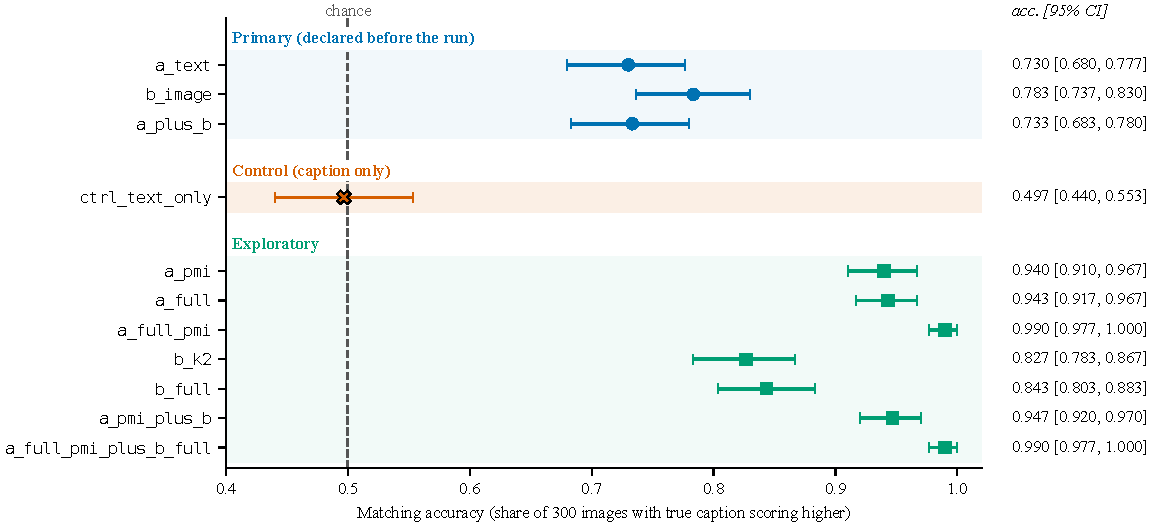
\includegraphics[width=0.92\linewidth]{figures/F1_probe1_accuracy.pdf}
\caption{Matching accuracy of UniDisc 1.4B on true versus mismatched COCO captions (exploratory feasibility result, 300 images).
Markers show the share of images for which the true caption scores higher (chance 0.5, dashed); bars are 95\,\% bootstrap intervals
over images (10\,000 resamples). Blue: primary scores, text direction a\_text and image direction b\_image with $K=8$ complementary
masks, and their sum. Orange: caption-only control, which stays at chance. Green: variants chosen after the primary results (image-masked
null subtracted, single full-mask pass, $K=2$, sums). One run, one mismatch draw; the intervals do not cover variation across draws or
models.}
\label{fig:probe1}
\end{figure}

\subsection{Hardware, runtime and missing items}\label{ssec:hardware}
All runs use one laptop GPU (12~GB) in short checkpointed chunks under a guard (Appendix~\ref{app:diag}).
Missing items are handled by a fixed rule: complete cases per analysis, no replacements and no reordering, so a crash leaves a
prefix of the item list; if the completed base fold has fewer than 240 items the paper says so, prints the minimum detectable effect
at the achieved $n$, and does not read ``not rejected'' as evidence against GATE-M.
No analysis that computes $Y$, $b$, $c$, $p$ or a difference of $d_R$ runs on test data before the planned fold is complete.
Mask-seed and corruption-seed variance are not in the intervals.

\subsection{Preregistration, pins and disclosed deviations}\label{ssec:prereg}
The code, the tests, the fold file, the hard-negative pool and the analysis plan are pinned by commit and SHA-256, and the pins,
the audit and sign-off record, the deviations known at the time of writing and the dated amendments are in Appendix~\ref{app:prereg}.
Changes after a pin are logged as dated amendments; none is made inside a stage.
% run: P2-GATE-CPU/m1_fallback
One analysis preceded the plan's second addendum and bears on the detection wording.
The first 21 items of the detection set were analysed on CPU without the gate statistic $q$, which needs a GPU pass.
In that exploratory look the mean per-item AUROC against changed-code labels of plain-$B$ was 0.54 on JPEG quality 10 and 0.51 on noise
0.10, while pixel variance with its sign flipped scored 0.76 and 0.77.
The sign of the pixel-variance rival therefore cannot be claimed to be fixed blind, which is why both signs of every rival are admitted
and the rival is chosen on the data.
\todo{AUTHOR: final list of amendments and the date of the first M2 outcome; confirm the status of the open decisions on guard
thresholds, the JPEG denoiser setting and the fallback before the run.}

\FloatBarrier

\section{Results}\label{sec:results}
% results.tex -- written 2026-10-29 from the frozen run files only (WRITER-RESULTS-1: research/paper2/benchmark/WRITER-RESULTS-1.md lists
% every number with its file and JSON key). Order: the primary family P first and alone as the headline; then the mechanism family and the
% evidence ratio; the denoising comparator; calibration and the clean control; the positive control on its own table; detection; E-dec and
% E-pred (AB.2, AB.3 wording); coherence; the families that are pending or not run; the exploratory Tier-3 comparison (A4.1.10 placement);
% the status of every family.
% Label of P (A4.2.1, mechanical from runs/P2-GATE-M3/family.json rule R2 and runs/P2-GATE-M4/analysis.json): NEG.
% AB.1: no sentence below uses PS, S-M, S-Z, S-DN, detection, E-dec, E-pred, S2, B, R, the suite or Tier 3 to explain, qualify or predict
% the P result. "predicted" appears only in the E-pred table header (AB.1 item 4).

\paragraph{Conventions for this section.}
Every interval is stated with its level.
Unless a caption says otherwise, intervals are paired percentile bootstrap intervals over items with 10\,000 resamples, and accuracy
means image-direction verification accuracy, the share of items whose true caption has the larger image-direction evidence
(Eq.~\eqref{eq:delta}; higher is better).
One emphasis rule holds for every table of this section: an estimate is set in bold when the interval in its row excludes zero (for the
exploratory accuracy contrasts of Tables~\ref{tab:res_tier3} and~\ref{tab:res_tier3_ps}, when the exact interval for the discordant
split excludes one half); nothing else is bold and nothing is underlined.
Every caption names the file and key that hold its numbers.

\subsection{Primary result: GATE-M against no gate (family P)}\label{ssec:res_primary}
% run: P2-GATE-M4 (analysis.json, primary.*, outcome.*); P2-GATE-M3 (family.json, n_rule.*)
In the preregistered test no improvement was detected under JPEG quality~10, Gaussian noise with $\sigma=0.10$ or a $128$-pixel splice.
For each tested corruption the 90\,\% interval of the net accuracy change lay inside $\pm0.05$: $-0.002$ ($-0.006$ to $0.000$) under
JPEG, $0.000$ ($0.000$ to $0.000$) under noise and $-0.004$ ($-0.010$ to $0.002$) under splice, with $n=500$ each, so an improvement
larger than 0.05 is excluded and a loss larger than 0.05 is excluded.
This is not a finding that GATE-M has no effect.
It holds in one pretrained unified masked diffusion model (UniDisc, 1.4B parameters) on COCO image-caption pairs with a random other
caption as the negative, at one severity per corruption.
By the pre-stated rule (Section~\ref{ssec:tests}) the label of the primary family is \emph{negative}: no hypothesis was rejected after
Holm correction over three, and every corruption had an operating point and 500 completed items.

Table~\ref{tab:res_primary} gives the full test.
The gate changed the decision on one of 500 items under JPEG, on none under noise and on four under splice, where it was right on one
and wrong on three ($b/n_d=0.25$, exact 95\,\% interval 0.006 to 0.806).
Under noise every bootstrap interval is the single point zero because no item was discordant; it records the absence of discordant
items, not a measured precision.
All 500 planned items of the test fold were completed, no item failed the caption-token check, and no arm had empty or non-finite
evidence.

\begin{table}[!tbp]
\centering
\caption{Primary family P: GATE-M against no gate on the 500 test items, image-direction verification accuracy (higher is better).
$b$: items right under GATE-M and wrong without a gate; $c$: the reverse; $n_d=b+c$.
Net difference $=(b-c)/n$, GATE-M minus none, with paired percentile bootstrap intervals over items (10\,000 resamples) at 90\,\%
(which carries the negative label), 95\,\% and 98.33\,\% (the Holm level of the first step).
$p$: exact two-sided McNemar test (Eq.~\eqref{eq:mcnemar}); $p_{\rm Holm}$: Holm over the three corruptions.
No estimate is bold: no interval excludes zero.
Source: \nolinkurl{runs/P2-GATE-M4/analysis.json}, keys \nolinkurl{primary.per_corruption.{jpeg,noise,splice}} and
\nolinkurl{outcome.label}.}
\label{tab:res_primary}
\footnotesize
\begin{adjustbox}{max width=\textwidth}
\begin{tabular}{lccccccc}
\toprule
Corruption & $n$ & Acc.\ none & Acc.\ GATE-M & $b$ & $c$ & Net diff. & $p$ ($p_{\rm Holm}$) \\
\midrule
JPEG, quality 10 & 500 & 0.838 & 0.836 & 0 & 1 & $-0.002$ & 1.00 (1.00) \\
& \multicolumn{7}{l}{\scriptsize intervals: 90\,\% $[-0.006,\,0.000]$; 95\,\% $[-0.006,\,0.000]$; 98.33\,\% $[-0.008,\,0.000]$} \\
Noise, $\sigma=0.10$ & 500 & 0.676 & 0.676 & 0 & 0 & $0.000$ & 1.00 (1.00) \\
& \multicolumn{7}{l}{\scriptsize intervals: 90\,\% $[0.000,\,0.000]$; 95\,\% $[0.000,\,0.000]$; 98.33\,\% $[0.000,\,0.000]$} \\
Splice, 128 px & 500 & 0.876 & 0.872 & 1 & 3 & $-0.004$ & 0.625 (1.00) \\
& \multicolumn{7}{l}{\scriptsize intervals: 90\,\% $[-0.010,\,0.002]$; 95\,\% $[-0.012,\,0.004]$; 98.33\,\% $[-0.014,\,0.004]$} \\
\bottomrule
\end{tabular}
\end{adjustbox}
\end{table}

\todo{RESULT FIGURE (A4.2.5, family P only): one row per corruption, net accuracy difference GATE-M minus none with the 90\,\% (thick)
and 95\,\% (thin) bootstrap intervals, a solid line at 0 and dashed lines at $\pm0.05$; nothing else on the canvas. Data:
\nolinkurl{runs/P2-GATE-M4/analysis.json}, \nolinkurl{primary.per_corruption.*.{delta,ci90,ci95}}.}

\paragraph{Operating points and sample size.}
% run: P2-GATE-M3 (family.json, rungs.*, n_rule.*, sensitivity_other_endpoint.z.*)
The operating points and the fold size were fixed on the 100 headroom items before any test item was scored (Section~\ref{ssec:headroom}).
The first rung of every corruption passed both headroom conditions (Table~\ref{tab:res_headroom}): JPEG quality~10, noise
$\sigma=0.10$ and the $128$-pixel splice.
The largest discordance between the changed-code gate and no gate among these rungs was $D^\ast=19$, which selects rule~R2: 500 test
items with the correctness endpoint.
On the headroom items JPEG quality~10 changed 986.7 of the 1\,024 codes of an image on average, noise 949.4 and the splice 237.2, and
the splice lowered the clean accuracy of the 100 headroom items by only 0.01.
On the size-scaled ratio $z_R$ of Eq.~\eqref{eq:dz}, a sensitivity analysis, the second condition fails at every rung ($T_2$ from
$-6.75$ to $-0.09$); the rule uses $d_R$.

\begin{table}[!tbp]
\centering
\caption{Headroom check on the 100 headroom items (no gate flag computed). $n_v$: items with all values; $T_1$, $T_2$: paired
$t$ statistics of clean minus corrupted and changed-code gate minus corrupted, on $d_R$; a rung passes if $n_v\ge90$, $T_1\ge2$ and
$T_2\ge2$, and the first passing rung is the operating point. $D_c$: items whose correctness differs between the changed-code gate
and no gate. Changed codes: mean number of the 1\,024 codes that differ from the clean tokenisation. Accuracy drop: clean minus
corrupted accuracy without a gate. Rungs after a passing first rung were computed but not used. No interval is reported, so nothing is
bold. $D^\ast=\max(19,18,2)=19$ over the operating points gives rule R2 ($18\le D^\ast<29$): 500 test items, endpoint $Y$.
Source: \nolinkurl{runs/P2-GATE-M3/family.json}, keys \nolinkurl{rungs.*} and \nolinkurl{n_rule.*}.}
\label{tab:res_headroom}
\footnotesize
\begin{adjustbox}{max width=\textwidth}
\begin{tabular}{lcccccccc}
\toprule
Rung & $n_v$ & $T_1$ & $T_2$ & Passes & $D_c$ & \makecell{Changed\\codes} & \makecell{Accuracy\\drop} & \makecell{Operating\\point} \\
\midrule
JPEG, quality 10 & 99 & 6.03 & 3.30 & yes & 19 & 986.7 & 0.06 & yes \\
JPEG, quality 5 & 95 & 5.16 & 1.54 & no & 26 & 1010.5 & 0.04 & -- \\
Noise, $\sigma=0.10$ & 100 & 4.20 & 4.38 & yes & 18 & 949.4 & 0.14 & yes \\
Noise, $\sigma=0.20$ & 100 & 3.79 & 4.27 & yes & 19 & 998.4 & 0.22 & -- \\
Splice, 128 px & 100 & 5.33 & 4.05 & yes & 2 & 237.2 & 0.01 & yes \\
Splice, 192 px & 100 & 7.93 & 7.34 & yes & 3 & 387.7 & 0.03 & -- \\
\bottomrule
\end{tabular}
\end{adjustbox}
\end{table}

\subsection{Mechanism controls (family S-M) and equal-size gates}\label{ssec:res_mech}
% run: P2-GATE-M4 (analysis.json, s_m.*, mechanism.<cell>.y.*, mechanism.<cell>.d.*)
Family S-M tests GATE-M against the geometry-matched random gate only on a corruption with a primary rejection with $b>c$; the others
keep $p=1$ in its Holm family of three.
There was no such corruption, so S-M tested no hypothesis, and its two pre-stated rules for an improvement that is not attributable to
detection do not apply.
The contrasts of GATE-M with the other gates of equal size are reported descriptively in Table~\ref{tab:res_mech}, with paired
bootstrap intervals and no $p$-value.
On every realistic corruption GATE-M was not distinguishable from the geometry-matched and the scattered random gates, each averaged
over its three seeds.
Under splice the top-$k$ gate on plain $B$, which removes the same number of tokens with the lowest uncalibrated likelihood, gave a
higher accuracy than GATE-M ($-0.008$, 95\,\% interval $-0.016$ to $-0.002$).
The changed-code gate, which keeps only the codes that the corruption left unchanged, lowered accuracy relative to no gate under
JPEG ($-0.084$, $-0.122$ to $-0.046$) and raised it under noise ($0.070$, $0.036$ to $0.104$).

\begin{table}[!tbp]
\centering
\caption{Equal-size gates on the 500 test items: accuracy of GATE-M minus each comparison gate, and of the changed-code gate minus no
gate, with paired percentile bootstrap 95\,\% intervals over items (10\,000 resamples). Geometry-matched and scattered random gates are
averaged over three seeds per item. Descriptive (exploratory); no $p$-value. Bold: the 95\,\% interval excludes zero.
Source: \nolinkurl{runs/P2-GATE-M4/analysis.json}, keys \nolinkurl{mechanism.{jpeg10,noise0.1,splice128}.y.*}.}
\label{tab:res_mech}
\footnotesize
\begin{adjustbox}{max width=\textwidth}
\begin{tabular}{lcccccc}
\toprule
& \multicolumn{5}{c}{GATE-M minus} & \\
\cmidrule(lr){2-6}
Corruption & \makecell{geometry-\\matched} & scattered & \makecell{plain-$B$\\top-$k$} & \makecell{$s_3$\\top-$k$} & \makecell{changed-\\code} & \makecell{Changed-code\\minus none} \\
\midrule
JPEG & $0.000$ & $-0.002$ & $0.000$ & $0.000$ & $\mathbf{0.082}$ & $\mathbf{-0.084}$ \\
& \scriptsize$[-0.002,0.002]$ & \scriptsize$[-0.007,0.001]$ & \scriptsize$[-0.006,0.006]$ & \scriptsize$[-0.008,0.008]$ & \scriptsize$[0.044,0.120]$ & \scriptsize$[-0.122,-0.046]$ \\
Noise & $0.001$ & $0.000$ & $-0.002$ & $0.000$ & $\mathbf{-0.070}$ & $\mathbf{0.070}$ \\
& \scriptsize$[0.000,0.002]$ & \scriptsize$[0.000,0.000]$ & \scriptsize$[-0.006,0.000]$ & \scriptsize$[0.000,0.000]$ & \scriptsize$[-0.104,-0.036]$ & \scriptsize$[0.036,0.104]$ \\
Splice & $-0.001$ & $-0.004$ & $\mathbf{-0.008}$ & $-0.006$ & $-0.008$ & $0.004$ \\
& \scriptsize$[-0.009,0.007]$ & \scriptsize$[-0.011,0.002]$ & \scriptsize$[-0.016,-0.002]$ & \scriptsize$[-0.016,0.002]$ & \scriptsize$[-0.022,0.006]$ & \scriptsize$[-0.010,0.018]$ \\
\bottomrule
\end{tabular}
\end{adjustbox}
\end{table}

\subsection{Evidence ratio (family S-Z)}\label{ssec:res_snr}
% run: P2-GATE-M4 (analysis.json, s_z.*, mechanism.<cell>.d.*, mechanism.<cell>.gate_on_clean.z)
GATE-M increased the evidence ratio $d_R$ of Eq.~\eqref{eq:dz} under all three corruptions (Wilcoxon signed-rank test, Holm over
three): by $0.0090$ (95\,\% interval $0.0078$ to $0.0102$; $p_{\rm Holm}=1.9\times10^{-39}$) under JPEG, by $0.0038$ ($0.0030$ to
$0.0047$; $8.5\times10^{-16}$) under noise and by $0.0078$ ($0.0069$ to $0.0087$; $2.9\times10^{-43}$) under splice.
This is not a result about verification accuracy.
The ratio rises when tokens with extreme per-token evidence are removed for any reason, and the plan states that the random gates do not
separate removing corrupted tokens from removing heavy-tailed ones.
Three descriptive contrasts bear on that caveat (paired bootstrap 95\,\% intervals, no $p$-value).
The geometry-matched random gate did not raise $d_R$: GATE-M minus that gate was $0.0091$ ($0.0078$ to $0.0104$), $0.0040$ ($0.0030$
to $0.0049$) and $0.0081$ ($0.0071$ to $0.0092$), close to GATE-M minus none.
The plain-$B$ top-$k$ gate raised $d_R$ almost as much as GATE-M (GATE-M minus it: $0.0008$, $0.0001$ to $0.0015$; $0.0003$, $-0.0001$
to $0.0007$; $0.0005$, $-0.0001$ to $0.0011$), and the $s_3$ top-$k$ gate less (GATE-M minus it: $0.0051$, $0.0035$ to $0.0067$;
$0.0033$, $0.0022$ to $0.0044$; $0.0045$, $0.0033$ to $0.0057$).
On the size-scaled $z_R$ (sensitivity endpoint, unadjusted Wilcoxon $p$) the change was $0.056$ ($0.025$ to $0.087$; $p=2.5\times10^{-4}$)
under JPEG, $0.011$ ($-0.012$ to $0.034$; $p=0.35$) under noise and $0.042$ ($0.017$ to $0.066$; $p=0.0012$) under splice, and on the
clean test images GATE-M raised $z_R$ by $0.058$ ($0.032$ to $0.085$).

\subsection{Pixel denoising as a defence (family S-DN)}\label{ssec:res_dn}
% run: P2-GATE-M4 (analysis.json, s_dn.*, mechanism.<cell>.denoise_minus_none.y)
Family S-DN compares GATE-M with no gate on a copy of the corrupted image cleaned by the pixel denoiser (exact McNemar, Holm over JPEG
and noise).
Under noise the denoised copy gave higher verification accuracy than GATE-M: 0.852 against 0.676 ($b=34$, $c=122$; GATE-M minus
denoised $-0.176$, 95\,\% interval $-0.224$ to $-0.130$; $p_{\rm Holm}=1.5\times10^{-12}$), against 0.880 on the clean images.
Under JPEG no difference was detected: 0.844 against 0.836 ($b=38$, $c=42$; $-0.008$, $-0.042$ to $0.026$; $p_{\rm Holm}=0.74$).
At this setting the denoiser lowers the quality of JPEG images (Section~\ref{ssec:baselines}), so the JPEG row compares GATE-M with a
defence that harms the image.
The denoised copy against no gate was $0.176$ ($0.130$ to $0.222$) under noise and $0.006$ ($-0.030$ to $0.040$) under JPEG.
Splice has no denoised copy.

\subsection{Calibration of the gate and the clean control (family S-C)}\label{ssec:res_cal}
% run: P2-GATE-M4 (analysis.json, calibration.fap_check.*, calibration.split_replication.*, calibration.per_condition.*, c1_test.*, s_c.*);
% run: P2-GATE-M2 (threshold.json thresholds.*.r_hat; c1_cal.json); P2-GATE-M3 (c1_head.json)
On the 500 clean test pairs the realised flagged share was 0.0456 at $\alpha=0.05$, with an item-bootstrap 95\,\% interval of 0.0442 to
0.0470 (Table~\ref{tab:res_cal}).
The calibration statistic was $-3.59$, against the violation bound of 2.13, so there is no evidence of violation; at $\alpha=0.01$ and
$0.10$ the shares were 0.0064 and 0.0956, also with no evidence of violation.
In 2\,000 random re-splits of calibration and test items at $\alpha=0.05$ (exploratory, descriptive) the mean of $\hat F-\alpha$ was
$-0.0031$, with 2.5 and 97.5 percentiles of $-0.0055$ and $-0.0006$.
The statement checked is the one of Proposition~\ref{prop:crc}, the expected flagged share of a clean pair's tokens; a pass is ``no
evidence of violation'' and not a validation.

\begin{table}[!tbp]
\centering
\caption{Clean false-alarm check on the 500 clean test pairs. $\hat F$: mean over items of the flagged share of an item's 1\,024
tokens; interval: percentile bootstrap 95\,\% over items (10\,000 resamples). $\hat F_{\rm cal}$: flagged share on the 300 calibration
pairs at the fitted threshold. $Z_{\rm cal}$: calibration statistic of Appendix~\ref{app:diagchecks}; a violation is flagged above 2.13. Nothing
is bold (no interval of a difference). Source: \nolinkurl{runs/P2-GATE-M4/analysis.json}, keys
\nolinkurl{calibration.fap_check.per_alpha.*}; \nolinkurl{runs/P2-GATE-M2/threshold.json}, keys \nolinkurl{thresholds.*.r_hat}.}
\label{tab:res_cal}
\footnotesize
\begin{tabular}{ccccc}
\toprule
$\alpha$ & $\hat F_{\rm cal}$ & $\hat F$ (test) [95\,\%] & $Z_{\rm cal}$ & Reading \\
\midrule
0.01 & 0.0067 & 0.0064 $[0.0061,\,0.0067]$ & $-16.12$ & no evidence of violation \\
0.05 & 0.0468 & 0.0456 $[0.0442,\,0.0470]$ & $-3.59$ & no evidence of violation \\
0.10 & 0.0970 & 0.0956 $[0.0928,\,0.0985]$ & $-1.76$ & no evidence of violation \\
\bottomrule
\end{tabular}
\end{table}

Table~\ref{tab:res_flags} gives, with equal prominence, what the guarantee does not cover: the false-alarm proportion on the unchanged
tokens of corrupted items, the hit rate on changed tokens and the precision among flagged tokens, at $\alpha=0.05$.
On the unchanged tokens of the realistic corruptions the false-alarm proportion was 0.036 to 0.044; under swap it was 0.089, above
$\alpha$.
Precision must be read against the share of changed tokens: under JPEG and noise more than nine in ten tokens change, so a precision of
0.976 and 0.922 is close to that base rate (0.961 and 0.928); under noise the hit rate (0.033) was below the false-alarm proportion
(0.036).

\begin{table}[!tbp]
\centering
\caption{Flags of the gate at $\alpha=0.05$ on the corrupted test images, token level, pooled over the 500 items. Changed share: share of
tokens whose code differs from the clean tokenisation ($\rho$). Hit rate: share of changed tokens flagged. False-alarm proportion:
share of unchanged tokens of corrupted items flagged (not covered by the guarantee). Precision: share of flagged tokens that changed.
Point estimates; no interval was computed, so nothing is bold. Patch and swap are the sanity corruptions of the positive control.
Source: \nolinkurl{runs/P2-GATE-M4/analysis.json}, keys \nolinkurl{calibration.per_condition.*.{precision,recall,fap_on_clean_tokens}}
and \nolinkurl{calibration.per_condition.*.prop4.rho}.}
\label{tab:res_flags}
\footnotesize
\begin{tabular}{lcccc}
\toprule
Corruption & Changed share & Hit rate & False-alarm proportion & Precision \\
\midrule
JPEG, quality 10 & 0.961 & 0.061 & 0.037 & 0.976 \\
Noise, $\sigma=0.10$ & 0.928 & 0.033 & 0.036 & 0.922 \\
Splice, 128 px & 0.227 & 0.049 & 0.044 & 0.248 \\
\midrule
Patch (sanity) & 0.062 & 0.750 & 0.050 & 0.498 \\
Swap (sanity) & 0.150 & 0.859 & 0.089 & 0.631 \\
\bottomrule
\end{tabular}
\end{table}

The clean no-gate accuracy on the test fold was 0.880 (Wilson 95\,\% interval 0.849 to 0.906), against 0.843 (0.798 to 0.880) in the
pilot; the intervals overlap, so the pre-stated pipeline audit was not triggered.
The same check gave 0.880 (0.838 to 0.912) on the calibration fold and 0.860 (0.779 to 0.915) on the headroom fold.
In the clean control (family S-C, exact McNemar, one hypothesis) GATE-M on clean images gave 0.882 against 0.880 without a gate ($b=2$,
$c=1$; net $0.002$, 95\,\% interval $-0.004$ to $0.010$; $p=1.00$): no change was detected.

\subsection{Positive control (family PS)}\label{ssec:res_ps}
% run: P2-GATE-M4 (analysis.json, ps.*)
The positive control repeats the primary test on the two sanity corruptions, with Holm correction over two (Table~\ref{tab:res_ps}).
Neither hypothesis was rejected, so the positive control was \emph{not met}.
By the plan this reads ``pipeline defect suspected, audit triggered''; nothing was tuned.
Both sanity corruptions lowered the clean accuracy of the test fold from 0.880 to 0.870 without a gate.
\todo{AUTHOR/RESULT: outcome of the pipeline audit triggered by the positive control (date, scope, result); until it is reported, a
pipeline defect is not excluded.}
The positive control says nothing about where the gate works.

\begin{table}[!tbp]
\centering
\caption{Positive control PS (pipeline check only): GATE-M against no gate on the sanity corruptions, 500 test items, image-direction
verification accuracy. Columns as in Table~\ref{tab:res_primary}: paired percentile bootstrap intervals over items (10\,000
resamples) at 95\,\% and 98.33\,\%; exact two-sided McNemar $p$; Holm over two. No estimate is bold: no interval excludes zero. Source:
\nolinkurl{runs/P2-GATE-M4/analysis.json}, keys \nolinkurl{ps.per_corruption.{patch,swap}} and \nolinkurl{ps.positive_control}.}
\label{tab:res_ps}
\footnotesize
\begin{adjustbox}{max width=\textwidth}
\begin{tabular}{lccccccc}
\toprule
Corruption & $n$ & Acc.\ none & Acc.\ GATE-M & $b$ & $c$ & Net diff. & $p$ ($p_{\rm Holm}$) \\
\midrule
Patch, $8\times8$ codes & 500 & 0.870 & 0.870 & 2 & 2 & $0.000$ & 1.00 (1.00) \\
& \multicolumn{7}{l}{\scriptsize intervals: 95\,\% $[-0.008,\,0.008]$; 98.33\,\% $[-0.010,\,0.010]$} \\
Swap, 15\,\% of codes & 500 & 0.870 & 0.876 & 8 & 5 & $0.006$ & 0.58 (1.00) \\
& \multicolumn{7}{l}{\scriptsize intervals: 95\,\% $[-0.008,\,0.020]$; 98.33\,\% $[-0.012,\,0.024]$} \\
\bottomrule
\end{tabular}
\end{adjustbox}
\end{table}

\subsection{Detection against cheap rivals (families S-D and S-D2)}\label{ssec:res_det}
% run: P2-GATE-M1
This family was analysed before the main test, on the 200 detection items, and it is a measurement of the within-modality score $q$;
it enters no claim about the primary result.
Intervals are 95\,\% percentile bootstrap intervals over items for the per-item AUROC against changed-code labels; items with too
few corrupted or clean tokens are excluded and counted (3 for JPEG, 2 for noise).
On the sanity corruptions $q$ reaches 0.961 (0.959 to 0.963) for a replaced patch and 0.955 (0.952 to 0.957) for swapped codes, so the
chance bar of the positive control was passed; plain-$B$ is slightly higher, 0.964 and 0.960, with $q$ minus plain-$B$ equal to
$-0.0033$ ($-0.0042$ to $-0.0026$) and $-0.0053$ ($-0.0058$ to $-0.0047$).
The non-finetuned TbV score reaches 0.854 and 0.859 and the neighbour codebook distance 0.786 and 0.741 on the same corruptions; a
check for copying of the released output layer suspected no item.
On JPEG quality 10 $q$ reaches 0.561 (0.547 to 0.575, 197 items) and on Gaussian noise 0.10 it reaches 0.503 (0.493 to 0.513, 198
items).
The non-finetuned TbV score reaches 0.581 (0.569 to 0.593) on JPEG and 0.607 (0.597 to 0.618) on noise; on noise the marginal
intervals of $q$ and TbV do not overlap, on JPEG they do, and no paired test between them was run.
The best cheap rival is the pixel variance of a token's patch with its sign flipped, 0.756 (0.743 to 0.768) on JPEG and 0.768 (0.760
to 0.776) on noise.
The rival and its sign were chosen on the data among about nine candidates, which biases the contrast against $q$.
The paired difference of $q$ minus the rival is $-0.195$ ($-0.214$ to $-0.175$) on JPEG and $-0.265$ ($-0.278$ to $-0.253$) on noise,
with a Holm-adjusted $p$ of 0.0004 on each, the resolution floor of 10\,000 resamples.
The result is the same when the rival is re-selected in every resample and when the 21 items analysed before the plan's second
addendum are removed (179 items).
The preregistered falsifier for the score was therefore met on both corruptions, and the paper does not say that the score detects
corrupted codes better than cheap methods.
That a texture score wins against this label is read as the label-circularity concern of Section~\ref{ssec:limits} and not as
evidence that texture explains the corruption effect.
Figure~\ref{fig:detection} shows the full detection map.

% run: P2-GATE-M4 (analysis.json, s_d2.*)
The out-of-sample family S-D2 repeats the contrast on the test items at the operating points, with the rival frozen on the complete
detection set (patch texture, sign flipped) and Holm correction over two.
Under JPEG quality~10 $q$ reached 0.561 against 0.759 for the rival (492 items with enough tokens of both kinds; $q$ minus rival
$-0.198$, 95\,\% interval $-0.211$ to $-0.186$; $p_{\rm Holm}=0.0004$), and under noise 0.509 against 0.767 (497 items; $-0.258$,
$-0.267$ to $-0.250$; $p_{\rm Holm}=0.0004$), again at the resolution floor.
S-D2 has no splice member, so the AUROC of $q$ under splice was not measured; its flag rates at $\alpha=0.05$ are in
Table~\ref{tab:res_flags}.

\begin{figure*}[!tbp]
\centering
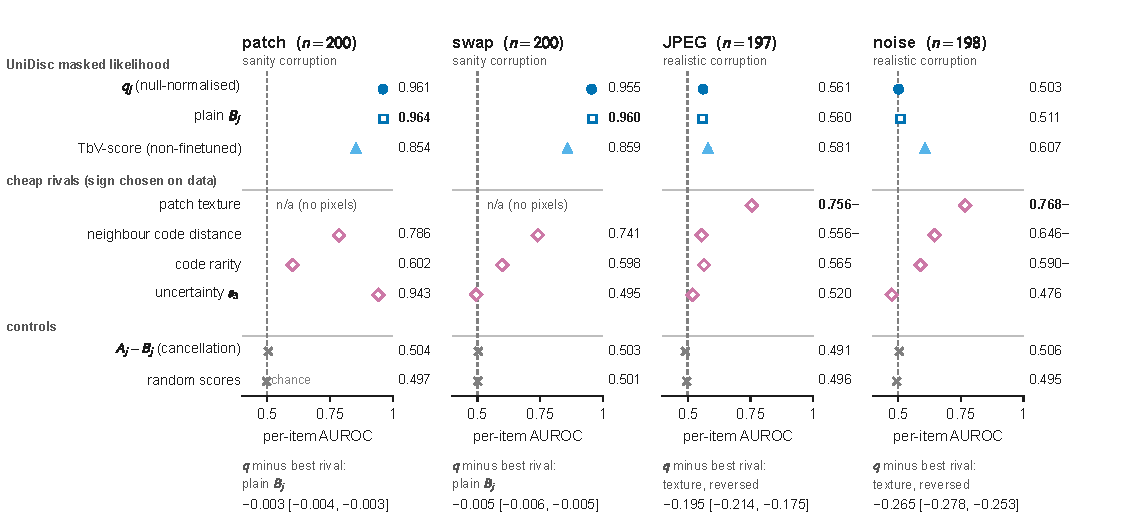
\includegraphics[width=\textwidth]{figures/F4_detection_map.pdf}
\caption{Detection map: per-item AUROC of each score against the changed-code labels, by corruption, on the 200 detection items
(secondary family S-D; not a test of the gate effect). Markers are the mean over items; bars are 95\,\% percentile bootstrap intervals over
items (10\,000 resamples), narrower than the marker for most rows; numbers at the right are the means (bold: highest in the panel).
$n$: items with enough corrupted and clean tokens (200 patch and swap, 197 JPEG, 198 noise); texture needs a pixel image and is not
applicable to patch and swap. Blue: the within-modality masked likelihood of UniDisc ($q_j$ and plain $B_j$); sky blue: TbV score,
non-finetuned. Reddish purple, hollow: cheap rivals, each in the better of its two orientations chosen on these data (a trailing minus
marks the reversed one), so rival values are optimistic. Grey: controls ($A_j-B_j$ and random scores); dashed line: chance, 0.5. Under
each panel: $q$ minus the best rival with its 95\,\% interval. No claim is made that $q$ detects better than the cheap rivals; the texture
result is a label-circularity concern, not an account of the corruption effect. Source: \nolinkurl{runs/P2-GATE-M1/analysis.json}, keys
\nolinkurl{table.*}, \nolinkurl{falsifier.per_corruption} and \nolinkurl{paired_q_vs_best_cheap}; script
\nolinkurl{paper2/figures/src/fig_detection_map.py}.}
\label{fig:detection}
\end{figure*}

\subsection{Decomposition of the accuracy lost to corruption (E-dec, descriptive)}\label{ssec:res_edec}
% run: P2-GATE-M4 (edec.json, cells.*)
E-dec splits the accuracy lost to corruption, $T=A_{\rm clean}-A_{\rm none}$, into the residual loss under the oracle gate
$U=A_{\rm clean}-A_{\rm chg}$, the realised recovery by GATE-M $R=A_{\rm GATE\text{-}M}-A_{\rm none}$ and the gap to the oracle gate
$V=A_{\rm chg}-A_{\rm GATE\text{-}M}$, so that $T=U+R+V$ item by item (Table~\ref{tab:res_edec}).
The oracle is the changed-code gate.
It is descriptive: no test, no $p$-value, and no part is an account of the primary result.
Under JPEG the gap to the oracle gate was negative with an interval that excludes zero ($V=-0.078$, $-0.116$ to $-0.040$), which by the
plan voids any detection reading of the JPEG cell.
Under noise the oracle gate recovered part of the loss ($V=0.070$, $0.036$ to $0.106$, of $T=0.204$).
Under splice the loss itself was not distinguishable from zero ($T=0.004$, $-0.006$ to $0.014$).
On the evidence ratio $d_R$ the same split gave $T=0.061$ ($0.048$ to $0.075$), $R=0.0090$ ($0.0078$ to $0.0101$), $V=0.073$ ($0.035$ to
$0.115$) under JPEG; $T=0.119$ ($0.099$ to $0.141$), $R=0.0038$ ($0.0030$ to $0.0047$), $V=0.083$ ($0.042$ to $0.116$) under noise;
and $T=0.020$ ($0.017$ to $0.023$), $R=0.0078$ ($0.0069$ to $0.0088$), $V=0.018$ ($0.014$ to $0.022$) under splice.
On the positive-control cells (accuracy scale) $T$ was $0.010$ ($0.002$ to $0.020$) for patch and $0.010$ ($-0.002$ to $0.022$) for swap,
with $R=0.000$ ($-0.008$ to $0.008$) and $0.006$ ($-0.008$ to $0.020$).
The parts are relative to the changed-code label, which marks encoder instability and is not an evidence oracle: $U$ contains a
composition effect, because the removed positions carry different evidence from the rest, and $V$ mixes false alarms, misses,
trimming of the variance and the shape of the gate.

\begin{table}[!tbp]
\centering
\caption{E-dec on the accuracy scale, primary cells (descriptive; no test). $T$: clean minus corrupted accuracy without a gate; $U$:
residual loss under the oracle (changed-code) gate; $R$: realised recovery by GATE-M; $V$: gap to the oracle gate; $T=U+R+V$.
Paired percentile bootstrap 95\,\% intervals over items, items resampled jointly (10\,000 resamples). $n$: complete items (two JPEG items
have no finite changed-code value). Bold: the 95\,\% interval excludes zero. Source: \nolinkurl{runs/P2-GATE-M4/edec.json}, keys
\nolinkurl{cells.{P1,P2,P3}.accuracy_scale.tau.*}.}
\label{tab:res_edec}
\footnotesize
\begin{adjustbox}{max width=\textwidth}
\begin{tabular}{lccccc}
\toprule
Cell & $n$ & $T$ & $U$ & $R$ & $V$ \\
\midrule
JPEG (P1) & 498 & $\mathbf{0.044}$ & $\mathbf{0.124}$ & $-0.002$ & $\mathbf{-0.078}$ \\
& & \scriptsize$[0.018,0.070]$ & \scriptsize$[0.088,0.161]$ & \scriptsize$[-0.006,0.000]$ & \scriptsize$[-0.116,-0.040]$ \\
Noise (P2) & 500 & $\mathbf{0.204}$ & $\mathbf{0.134}$ & $0.000$ & $\mathbf{0.070}$ \\
& & \scriptsize$[0.166,0.244]$ & \scriptsize$[0.098,0.172]$ & \scriptsize$[0.000,0.000]$ & \scriptsize$[0.036,0.106]$ \\
Splice (P3) & 500 & $0.004$ & $0.000$ & $-0.004$ & $0.008$ \\
& & \scriptsize$[-0.006,0.014]$ & \scriptsize$[-0.016,0.016]$ & \scriptsize$[-0.012,0.004]$ & \scriptsize$[-0.006,0.024]$ \\
\bottomrule
\end{tabular}
\end{adjustbox}
\end{table}

\subsection{Sign agreement of the independent-token calculation (E-pred, descriptive)}\label{ssec:res_epred}
% run: P2-GATE-M4 (epred_score.json, cells.*, P.*, PS.*); P2-GATE-EPRED-FIT (frozen signs, committed before the first M4 item)
E-pred compares, cell by cell, the sign $s_c$ of the plug-in signal-to-noise change of Eq.~\eqref{eq:snr}, fixed on a separate fit chunk
and committed before the first test item, with the observed sign $o_c$ of the net accuracy difference $b-c$ (Table~\ref{tab:res_epred}).
It has no test, no $p$-value and no level.
On the primary cells the sign of the plug-in signal-to-noise change agreed with the sign of the net accuracy difference in 2 of 2 cells
(95\,\% Clopper--Pearson interval 0.158 to 1.000); the noise cell had no observed sign ($b=c=0$) and was excluded.
The rival rule ``always $+$'' agreed in 0 of 2 cells and the rule ``$-$ for primary cells, $+$ for positive-control cells'' in 2 of 2.
On the positive-control cells, whose outcome was foregone by design, the signs agreed in 0 of 1 (0.000 to 0.975); the patch cell had
no observed sign.
No cell had an observed interval that excludes zero, so the refutation rule of the plan (a sign that disagrees with such a cell) was
not met in any cell.
The analysis file also records the comparison on the evidence ratio $d_R$, which GATE-M raised in all three primary cells with
intervals that exclude zero (Section~\ref{ssec:res_snr}) while the plug-in sign was negative; the plan fixes the observed sign on
correctness, and $d_R$ rises when extreme tokens are removed for any reason, so this disagreement is reported and not read either way.
The plug-in estimates on the test fold were, for JPEG, noise and splice: changed share $\rho$ 0.961, 0.928, 0.227; clean-token mean
$\mu$ 0.213, 0.182, 0.202 and variance $\sigma^2$ 0.501, 0.431, 0.510; changed-token mean $\mu_c$ 0.169, 0.099, 0.132 and variance
$\sigma_c^2$ 0.556, 0.456, 0.492; false-alarm rate $\hat\phi_0$ 0.037, 0.036, 0.044; hit rate $\hat\phi_1$ 0.061, 0.033, 0.049.

\begin{table}[!tbp]
\centering
\caption{E-pred, primary cells (descriptive; family E withdrawn, no test). $s_c$: committed sign of the plug-in signal-to-noise change
(Eq.~\eqref{eq:snr}) from the fit chunk, with the share of fit resamples giving the same sign; $o_c$: sign of $b-c$ for GATE-M against
none; $o_c^\ast$: the same sign only where the 95\,\% paired bootstrap interval of the net difference excludes zero. Net difference with
its paired percentile bootstrap 95\,\% interval over items. Agreement $A/K_{\rm eval}=2/2$ (Clopper--Pearson 95\,\% interval 0.158 to
1.000); rival rules: ``always $+$'' 0/2, ``$-$ for primary cells, $+$ for positive-control cells'' 2/2. No estimate is bold: no
interval excludes zero. Positive-control cells are reported in the text. Source: \nolinkurl{runs/P2-GATE-M4/epred_score.json}, keys \nolinkurl{cells.{P1,P2,P3}} and \nolinkurl{P}.}
\label{tab:res_epred}
\footnotesize
\begin{adjustbox}{max width=\textwidth}
\begin{tabular}{lcccccccc}
\toprule
Cell & \makecell{predicted\\sign $s_c$} & \makecell{Same-sign\\share} & $b$ & $c$ & \makecell{Net diff.\\{[95\,\%]}} & \makecell{observed\\sign $o_c$} & $o_c^\ast$ & Agree \\
\midrule
JPEG (P1) & $-$ & 1.000 & 0 & 1 & $-0.002$ & $-$ & none & yes \\
& & & & & \scriptsize$[-0.006,0.000]$ & & & \\
Noise (P2) & $-$ & 1.000 & 0 & 0 & $0.000$ & none & none & \makecell{excluded\\($b=c$)} \\
& & & & & \scriptsize$[0.000,0.000]$ & & & \\
Splice (P3) & $-$ & 1.000 & 1 & 3 & $-0.004$ & $-$ & none & yes \\
& & & & & \scriptsize$[-0.012,0.004]$ & & & \\
\bottomrule
\end{tabular}
\end{adjustbox}
\end{table}

\subsection{Re-infilling the flagged tokens (family S2)}\label{ssec:res_s2}
\todo{RESULT (run P2-GATE-S2; pending): status ``run, formal'', ``run, descriptive ($n<120$)'', ``partial prefix'' or ``not run'' with the
reason. If run: patch and splice, I-GATE against I-RAND4 (kept draw, exact McNemar, Holm over two) with the draw-level and all-four
contrasts beside it and I-GATE against none printed beside it; completed $n$. The claim-bearing cell is splice; a patch-only rejection
is a positive control with no realistic cell. No statement for JPEG or noise; the string ``G.1'' is not used. No sentence relates S2 to
the primary result (AB.1).}

\subsection{Two-way fusion on hard negatives (family B)}\label{ssec:res_text}
\todo{RESULT (run P2-GATE-FOIL; pending): status ``run, formal'', ``untestable at ceiling'' (with the clean accuracy of the better single
direction on the fit pairs) or ``not run'' with the reason. If run: fusion against the better single direction (exact McNemar, one
hypothesis), the two margins and the frozen fusion line; text-direction conditioning arms for the three realistic corruptions with
intervals (exploratory). B says nothing about corruption and nothing about the primary result (AB.1). If B ran before S2, state the
logged order and the inversion risk.}

\subsection{Second model (family R)}\label{ssec:res_omni}
Family R was not run.
It is gatekept by the primary family: it repeats the primary test on a second model only for corruptions with a primary rejection with
$b>c$, and there was none.

\subsection{Exploratory corruption suite}\label{ssec:res_suite}
\todo{RESULT (pending): the exploratory corruption suite (eight cells, intervals only, no $p$-value in any claim), or ``not run'' with the
reason; never in the abstract or highlights and never pooled with E-pred.}

\subsection{Exploratory: hard gate against detector-free combiners, discounting and reliability weighting of the same evidence}\label{ssec:res_expl}
% run: P2-GATE-M4 (tier3_fusion.json; run once after analysis.json with the P section was committed; SAP Addendum A4 r3, A4.1)
This comparison was pre-specified in Addendum A4 (Section~\ref{ssec:tier3}) and is exploratory (Tier~3): intervals only, no $p$-value,
72 intervals in all and no multiplicity adjustment.
It was run once, after the primary analysis was committed, on the same per-token evidence $\Delta_j$, items and decision rule as the
primary family, and it cannot explain, qualify or rescue the primary result.
Each comparator is contrasted with the hard gate (GM, which is GATE-M) on the same items.
The reading of a contrast comes from the exact Clopper--Pearson 95\,\% interval for the share $b/n_d$ of discordant items won by the
comparator: \emph{above} GM if its lower end exceeds one half, \emph{below} if its upper end is under one half, \emph{identical} if
$n_d=0$, and \emph{not distinguishable} otherwise.
Beside it are printed the net difference with a percentile bootstrap 95\,\% interval (descriptive) and the bound used for added value:
for $n_d<10$ the exact 95\,\% upper bound $B$ on the discordance rate, which bounds the absolute net difference, and for $n_d\ge10$ the
minimum detectable difference (MDD, two-sided 5\,\%, 80\,\% power, at the realised spread).
Tables~\ref{tab:res_tier3} and~\ref{tab:res_tier3_ps} give every cell and every comparator.

On the realistic corruptions no detector-free combiner gave higher verification accuracy than the hard gate.
The hard gate gave higher verification accuracy than the median under JPEG ($-0.032$, 95\,\% interval $-0.052$ to $-0.014$; exact
95\,\% interval for the discordant split 0.047 to 0.374) and under splice ($-0.032$, $-0.050$ to $-0.016$; 0.001 to 0.273), and higher
than the 20\,\% trimmed mean under JPEG ($-0.020$, $-0.034$ to $-0.006$; 0.018 to 0.428) and splice ($-0.026$, $-0.040$ to $-0.014$;
0.000 to 0.247); all exploratory.
The data do not show a difference between the hard gate and the trimmed mean at the gate's flag count under JPEG ($-0.002$, $-0.010$ to
$0.006$; $n_d=5$; $B=0.023$), noise ($0.000$, $-0.006$ to $0.006$; $n_d=2$; $B=0.014$) or splice ($-0.006$, $-0.014$ to $0.000$; $n_d=3$;
$B=0.017$), nor, under noise, between the hard gate and the median ($0.002$, $-0.016$ to $0.020$; $n_d=19$; MDD 0.025) or the 20\,\%
trimmed mean ($0.006$, $-0.006$ to $0.018$; $n_d=9$; $B=0.034$); all exploratory.
Because each of these bounds is at most 0.05, each counts, by the pre-stated rule, as a finding against the added value of the detector
over a detector-free combiner on that cell; by limit~(c) below, the contrast with the trimmed mean at the gate's flag count largely
repeats the primary contrast when the gate's score is near chance.
Discarding and discounting the gate-flagged tokens were not distinguishable under JPEG ($n_d=1$, $B=0.011$) or splice ($n_d=2$,
$B=0.014$), and made the same decision on all 500 items under noise ($n_d=0$; the net difference in accuracy is at most 0.007, exact
95\,\% bound on the discordance rate).
Discarding and reliability weighting of every token were not distinguishable on any realistic corruption ($n_d=15$, 18 and 12; MDD 0.022,
0.024 and 0.020).
Against no gate, no comparator gave higher accuracy on a realistic corruption; the median and the 20\,\% trimmed mean gave lower
accuracy than no gate under JPEG and splice, and on clean pairs too (exact readings; keys \nolinkurl{contrasts.*_minus_NONE} of the
same file).

On the evidence ratio $d_R$ (descriptive control of the plan) the trimmed mean at the gate's flag count gave a higher $d_R$ than the
hard gate on every cell: by $0.033$ (95\,\% interval $0.028$ to $0.039$) under JPEG, $0.018$ ($0.014$ to $0.022$) under noise, $0.031$
($0.027$ to $0.035$) under splice and $0.033$ ($0.029$ to $0.038$) on clean pairs, and the 20\,\% trimmed mean by $0.259$ ($0.225$ to
$0.292$), $0.195$ ($0.153$ to $0.237$), $0.303$ ($0.270$ to $0.334$) and $0.324$ ($0.291$ to $0.356$); exploratory.
Symmetric trimming lowers the spread of the retained evidence mechanically, which is why this control was specified.

On the positive-control cells (Table~\ref{tab:res_tier3_ps}; pipeline check only) reliability weighting of every token gave higher
verification accuracy than the hard gate under swap ($0.016$, 95\,\% interval $0.004$ to $0.030$; exact 95\,\% interval for the
discordant split 0.516 to 0.979; exploratory) and than no gate ($0.022$, $0.006$ to $0.038$; 0.566 to 0.962); this concerns discarding
against weighting on a sanity corruption and is not a finding about the realistic corruptions.

\begin{table}[!tbp]
\centering
\caption{Exploratory (Tier 3): the hard gate GM (GATE-M) against detector-free combiners (MED: median; TM-G: trimmed mean removing
$\lfloor g_i/2\rfloor$ tokens from each tail, $g_i$ the gate's flag count; TM20: 20\,\% trimmed mean), discounting of the gate-flagged
tokens (SOFT-G) and reliability weighting of every token (SOFT-A), on the same $\Delta_j$ and items ($n=500$ per cell; primary cells and
the clean cell). Acc.: accuracy of the comparator. $b$/$c$: items right only under the comparator / only under GM. $\Delta$: comparator
minus GM with its percentile bootstrap 95\,\% interval (descriptive; 10\,000 resamples, one index matrix per cell). Exact: Clopper--Pearson
95\,\% interval for $b/n_d$, which gives the reading. Bound: $B$ (exact 95\,\% upper bound on the discordance rate) for $n_d<10$, MDD for
$n_d\ge10$. Reading: above or below GM, not distinguishable (n.d.) or identical; $\dagger$: counts as a finding against the added value
of the detector (n.d.\ or identical for a detector-free combiner with bound at most 0.05; primary cells only). Bold: the exact interval excludes one half. 72 intervals in this
comparison; no $p$-value and no multiplicity adjustment. Limits: (a) no sign-aware detector-free estimator is computed, because the
direction in which a corruption moves $\Delta_j$ is defined by the true caption and such a combiner would use the label; (b) SOFT-G's
weights lie token by token between GM's and no gate's, so it is not reliability weighting of every token; (c) when the gate's score is
near chance the flagged count is close to the false-alarm count, so TM-G approximates no gate trimmed at about that count and TM-G
minus GM largely repeats the primary contrast; (d) at this $n$ many contrasts are uninformative, as the bound shows. Source:
\nolinkurl{runs/P2-GATE-M4/tier3_fusion.json}, keys \nolinkurl{cells.*.arms}, \nolinkurl{cells.*.contrasts.*_minus_GM},
\nolinkurl{clean.arms}, \nolinkurl{clean.contrasts}.}
\label{tab:res_tier3}
\footnotesize
\begin{adjustbox}{max width=\textwidth}
\begin{tabular}{llccccccl}
\toprule
Cell & Comparator & Acc. & $b$/$c$ & $n_d$ & $\Delta$ [95\,\%, descriptive] & Exact 95\,\% & Bound & Reading \\
\midrule
\multicolumn{9}{l}{JPEG, quality 10 \quad (GM 0.836; no gate 0.838; mean flagged tokens 61.8)} \\
& MED & 0.804 & 4/20 & 24 & $\mathbf{-0.032}$ $[-0.052,-0.014]$ & 0.047--0.374 & MDD 0.027 & below GM \\
& TM-G & 0.834 & 2/3 & 5 & $-0.002$ $[-0.010,0.006]$ & 0.053--0.853 & $B$ 0.023 & n.d.$^{\dagger}$ \\
& TM20 & 0.816 & 2/12 & 14 & $\mathbf{-0.020}$ $[-0.034,-0.006]$ & 0.018--0.428 & MDD 0.021 & below GM \\
& SOFT-G & 0.838 & 1/0 & 1 & $0.002$ $[0.000,0.006]$ & 0.025--1.000 & $B$ 0.011 & n.d. \\
& SOFT-A & 0.838 & 8/7 & 15 & $0.002$ $[-0.014,0.018]$ & 0.266--0.787 & MDD 0.022 & n.d. \\
\midrule
\multicolumn{9}{l}{Noise, $\sigma=0.10$ \quad (GM 0.676; no gate 0.676; mean flagged tokens 33.9)} \\
& MED & 0.678 & 10/9 & 19 & $0.002$ $[-0.016,0.020]$ & 0.289--0.756 & MDD 0.025 & n.d.$^{\dagger}$ \\
& TM-G & 0.676 & 1/1 & 2 & $0.000$ $[-0.006,0.006]$ & 0.013--0.987 & $B$ 0.014 & n.d.$^{\dagger}$ \\
& TM20 & 0.682 & 6/3 & 9 & $0.006$ $[-0.006,0.018]$ & 0.299--0.925 & $B$ 0.034 & n.d.$^{\dagger}$ \\
& SOFT-G & 0.676 & 0/0 & 0 & $0.000$ & -- & $B$ 0.007 & identical \\
& SOFT-A & 0.676 & 9/9 & 18 & $0.000$ $[-0.016,0.016]$ & 0.260--0.740 & MDD 0.024 & n.d. \\
\midrule
\multicolumn{9}{l}{Splice, 128 px \quad (GM 0.872; no gate 0.876; mean flagged tokens 46.0)} \\
& MED & 0.840 & 1/17 & 18 & $\mathbf{-0.032}$ $[-0.050,-0.016]$ & 0.001--0.273 & MDD 0.024 & below GM \\
& TM-G & 0.866 & 0/3 & 3 & $-0.006$ $[-0.014,0.000]$ & 0.000--0.708 & $B$ 0.017 & n.d.$^{\dagger}$ \\
& TM20 & 0.846 & 0/13 & 13 & $\mathbf{-0.026}$ $[-0.040,-0.014]$ & 0.000--0.247 & MDD 0.020 & below GM \\
& SOFT-G & 0.876 & 2/0 & 2 & $0.004$ $[0.000,0.010]$ & 0.158--1.000 & $B$ 0.014 & n.d. \\
& SOFT-A & 0.880 & 8/4 & 12 & $0.008$ $[-0.006,0.022]$ & 0.349--0.901 & MDD 0.020 & n.d. \\
\midrule
\multicolumn{9}{l}{Clean pairs, cost of each combiner \quad (GM 0.882; no gate 0.880; mean flagged tokens 46.7)} \\
& MED & 0.852 & 1/16 & 17 & $\mathbf{-0.030}$ $[-0.046,-0.014]$ & 0.001--0.287 & MDD 0.023 & below GM \\
& TM-G & 0.874 & 1/5 & 6 & $-0.008$ $[-0.018,0.000]$ & 0.004--0.641 & $B$ 0.026 & n.d. \\
& TM20 & 0.854 & 0/14 & 14 & $\mathbf{-0.028}$ $[-0.044,-0.014]$ & 0.000--0.232 & MDD 0.021 & below GM \\
& SOFT-G & 0.880 & 0/1 & 1 & $-0.002$ $[-0.006,0.000]$ & 0.000--0.975 & $B$ 0.011 & n.d. \\
& SOFT-A & 0.884 & 6/5 & 11 & $0.002$ $[-0.012,0.014]$ & 0.234--0.833 & MDD 0.019 & n.d. \\
\bottomrule
\end{tabular}
\end{adjustbox}
\end{table}

\begin{table}[!tbp]
\centering
\caption{Exploratory (Tier 3), positive-control cells only (pipeline check; never pooled with or shown beside the primary cells).
Columns, comparators, bound, reading and bold rule as in Table~\ref{tab:res_tier3}; $n=500$ per cell; ``against added value'' is not
read on these cells. Source: \nolinkurl{runs/P2-GATE-M4/tier3_fusion.json}, keys \nolinkurl{ps_cells.{patch,swap}.arms} and
\nolinkurl{ps_cells.{patch,swap}.contrasts.*_minus_GM}.}
\label{tab:res_tier3_ps}
\footnotesize
\begin{adjustbox}{max width=\textwidth}
\begin{tabular}{llccccccl}
\toprule
Cell & Comparator & Acc. & $b$/$c$ & $n_d$ & $\Delta$ [95\,\%, descriptive] & Exact 95\,\% & Bound & Reading \\
\midrule
\multicolumn{9}{l}{Patch \quad (GM 0.870; no gate 0.870; mean flagged tokens 96.5)} \\
& MED & 0.846 & 2/14 & 16 & $\mathbf{-0.024}$ $[-0.040,-0.010]$ & 0.016--0.383 & MDD 0.022 & below GM \\
& TM-G & 0.858 & 2/8 & 10 & $-0.012$ $[-0.024,0.000]$ & 0.025--0.556 & MDD 0.018 & n.d. \\
& TM20 & 0.846 & 2/14 & 16 & $\mathbf{-0.024}$ $[-0.040,-0.010]$ & 0.016--0.383 & MDD 0.022 & below GM \\
& SOFT-G & 0.870 & 0/0 & 0 & $0.000$ & -- & $B$ 0.007 & identical \\
& SOFT-A & 0.880 & 8/3 & 11 & $0.010$ $[-0.002,0.024]$ & 0.390--0.940 & MDD 0.018 & n.d. \\
\midrule
\multicolumn{9}{l}{Swap \quad (GM 0.876; no gate 0.870; mean flagged tokens 209.7)} \\
& MED & 0.838 & 1/20 & 21 & $\mathbf{-0.038}$ $[-0.056,-0.020]$ & 0.001--0.238 & MDD 0.025 & below GM \\
& TM-G & 0.852 & 1/13 & 14 & $\mathbf{-0.024}$ $[-0.040,-0.010]$ & 0.002--0.339 & MDD 0.021 & below GM \\
& TM20 & 0.846 & 0/15 & 15 & $\mathbf{-0.030}$ $[-0.046,-0.016]$ & 0.000--0.218 & MDD 0.021 & below GM \\
& SOFT-G & 0.878 & 2/1 & 3 & $0.002$ $[-0.004,0.010]$ & 0.094--0.992 & $B$ 0.017 & n.d. \\
& SOFT-A & 0.892 & 10/2 & 12 & $\mathbf{0.016}$ $[0.004,0.030]$ & 0.516--0.979 & MDD 0.019 & above GM \\
\bottomrule
\end{tabular}
\end{adjustbox}
\end{table}

\subsection{Coherence of the denoiser across mask patterns}\label{ssec:res_coh}
% run: P2-GATE-M5 (coherence.json; mu_from_m4.json)
On 100 clean calibration items, with four image-token pairs per item and two visible contexts per pair (800 gaps), the median absolute
order gap of the joint log-likelihood was 0.071 nats.
The same computation repeated in a different batch order on 25 items gave a 95th percentile of 0.000 for the 200 absolute repeat
differences, so at least 95 percent of the repeats reproduced the original value exactly.
Neither pre-stated reading applies.
The gap exceeds the numerical noise floor, so the denoiser is not ``coherent within numerical noise''; it is below the clean mean
per-token paired evidence $\mu=0.199$ measured on the 500 clean test items, so it is not ``incoherent at the evidence scale'', and
Eq.~\eqref{eq:marginalise} is not declared inapplicable.
By pair type (descriptive, not a pre-stated reading) the median gap was 0.253 for horizontally adjacent tokens, 0.246 for vertically
adjacent ones and 0.032 for distant ones; the two adjacent medians exceed $\mu$.

\subsection{Status of every family and cost}\label{ssec:res_cost}
Table~\ref{tab:res_status} gives the status of every family; a status is set by time and by the gatekeeping rules, never by an outcome.

\begin{table}[!tbp]
\centering
\caption{Status of every family and analysis of the main run (status only, no estimate). Nothing is bold. Sources: the run files cited in
each subsection of Section~\ref{sec:results}.}
\label{tab:res_status}
\footnotesize
\begin{tabular}{p{0.2\linewidth}p{0.42\linewidth}p{0.26\linewidth}}
\toprule
Family or analysis & Status & Section \\
\midrule
P (headline) & run, formal; $n=500$ (rule R2); label negative & \ref{ssec:res_primary} \\
S-M & run; no hypothesis tested (gatekept: no primary rejection with $b>c$) & \ref{ssec:res_mech} \\
S-Z & run, formal & \ref{ssec:res_snr} \\
S-DN & run, formal & \ref{ssec:res_dn} \\
S-C & run, formal & \ref{ssec:res_cal} \\
PS & run, formal; positive control not met (audit triggered) & \ref{ssec:res_ps} \\
S-D, S-D2 & run, formal; falsifier for the score met & \ref{ssec:res_det} \\
E-dec, E-pred & run, descriptive & \ref{ssec:res_edec}, \ref{ssec:res_epred} \\
S2 & \todo{RESULT: status} & \ref{ssec:res_s2} \\
B & \todo{RESULT: status} & \ref{ssec:res_text} \\
R & not run (gatekept: no primary rejection with $b>c$) & \ref{ssec:res_omni} \\
Suite & \todo{RESULT: status} & \ref{ssec:res_suite} \\
Tier 3 comparison & run, exploratory (intervals only) & \ref{ssec:res_expl} \\
Coherence check & run, pipeline check; neither pre-stated reading & \ref{ssec:res_coh} \\
\bottomrule
\end{tabular}
\end{table}

\todo{RESULT: network passes per item by stage, median time per item and peak GPU memory, from the run configuration and telemetry files
of runs P2-GATE-M2 to M5 (not yet extracted). The operational stops of the main run are in the deviations box (Appendix~\ref{app:deviations}).}

\FloatBarrier

\section{Discussion and limitations}\label{sec:discussion}
% discussion.tex -- Findings written 2026-10-29 for the label NEG of P (SAP Addendum A4, A4.2.3: opening of 6.1 near-verbatim).
% The fusion-context and limitations subsections are outcome-independent and drafted from the preregistration (card v4, SAP, A4).
% No sentence in this file draws on PS, S2, B, R, E-dec, E-pred, the suite, detection or the exploratory comparison to explain, qualify
% or predict the primary result (AB.1). The phrase "when does input gating help" is not used (D18 reading 1, decisions D0076-D0077);
% after the opening, the question of when gating can help is discussed only through the closed-form condition and the P table.
% Proposition 2 (correlated tokens) is not used on E-pred (D0078); Proposition 1 of the theory addendum is not used (D0078-D0079).

\subsection{Findings}\label{ssec:disc_findings}
% run: P2-GATE-M4 (analysis.json primary.*)
The preregistered test excludes an improvement or a loss of more than five percentage points in image-direction verification accuracy
from gating under JPEG quality~10, Gaussian noise with $\sigma=0.10$ and a $128$-pixel splice, for this model and these severities; it
does not show that gating has no effect.

The primary table shows how narrow the measured change is: in 500 items the gate changed the decision once under JPEG, never under
noise and four times under splice (Table~\ref{tab:res_primary}).
The exclusion of $\pm0.05$ is a statement about these discordances at the threshold calibrated for $\alpha=0.05$, at one severity per
corruption, in one model and on one data set.
It says nothing about a gate that flags a larger share of tokens, about stronger corruptions, or about another model or task, none of
which was tested.
Section~\ref{ssec:evidence} gives, under independent tokens, the condition on the hit and false-alarm rates under which discarding
flagged tokens raises the signal-to-noise ratio of an additive evidence sum (Eq.~\eqref{eq:snr}).
The condition states what a gate would have to achieve; it is an approximation for dependent image tokens, the test was not designed to
check it, and we do not use it to account for the result.

The remaining findings are separate measurements, each under its own family label, and none of them is an account of the primary result.
For each we give the observation, a hypothesis for it, and what would falsify the hypothesis.

\emph{The clean false-alarm statement held; the flags on corrupted images are not covered by it.}
% run: P2-GATE-M4 (calibration.*)
On held-out clean pairs the realised flagged share was 0.0456 at $\alpha=0.05$ (95\,\% interval 0.0442 to 0.0470), with no evidence
of violation at any of the three levels (Section~\ref{ssec:res_cal}).
On the unchanged tokens of corrupted images the false-alarm proportion was 0.036 to 0.044 for the realistic corruptions and 0.089 under
swap, above $\alpha$.
Hypothesis: a token next to a replaced code is scored with damaged context and is flagged more often, as Section~\ref{ssec:calibration}
anticipates.
It would be falsified if, under swap, the false-alarm proportion of an unchanged token did not fall with its distance to the nearest
replaced code; this was not measured.

\emph{The gate's score was near chance at finding the codes that JPEG and noise change.}
% run: P2-GATE-M1; P2-GATE-M4 (s_d2.*, calibration.per_condition.*)
On the detection items and again on the test items (families S-D and S-D2) the per-item AUROC of $q$ was 0.561 under JPEG and 0.503 and
0.509 under noise, below a texture score whose sign was chosen on the data; under noise the hit rate of the gate (0.033) was below its
false-alarm proportion on unchanged tokens (0.036).
Hypothesis, the label-circularity concern of Section~\ref{ssec:limits}: JPEG quality~10 and noise change more than nine in ten codes of
an image (Table~\ref{tab:res_flags}), so a changed code marks where the tokenizer is unstable more than where the image is damaged, and a
texture score tracks that instability.
It would be falsified if $q$ stayed at chance against a damage label defined in the pixel domain, for example the reconstruction error
of each token's patch, under which texture had no advantage; this was not measured.

\emph{A pixel denoiser restored most of the accuracy lost to noise.}
% run: P2-GATE-M4 (s_dn.*, c1_test.accuracy)
Under noise the denoised copy reached 0.852 against 0.676 without a gate and 0.880 on clean images, and it gave higher verification
accuracy than GATE-M (family S-DN, Section~\ref{ssec:res_dn}); under JPEG no difference was detected, with a denoiser setting that
lowers JPEG image quality.
Hypothesis: noise of this strength is largely removed in the pixel domain before tokenisation, so the tokens of the denoised image are
close to the clean ones.
It would be falsified if the share of codes that differ from the clean tokenisation were not lower for the denoised noisy images than for
the noisy ones; this was not measured.
The denoiser is a measured comparator, not part of the gate, and one setting was used.

\emph{Withholding every changed code lowered accuracy under JPEG.}
% run: P2-GATE-M4 (mechanism.jpeg10.y.changed_code_minus_none; edec.json cells.P1; calibration.per_condition.jpeg10.prop4.rho)
The changed-code gate, which keeps only the codes that the corruption left unchanged, lowered accuracy under JPEG by 0.084 and raised it
under noise by 0.070 (Table~\ref{tab:res_mech}); in E-dec the gap to this oracle was negative under JPEG with an interval that excludes
zero, which by the plan voids any detection reading of that cell (Section~\ref{ssec:res_edec}).
Hypothesis: under JPEG this gate decides on about four percent of the tokens of an image, and the sum over so few tokens is noisier than
the sum over all of them, which is the composition effect named in the plan.
It would be falsified if keeping a random set of the same small size, instead of the unchanged codes, did not lower accuracy by a similar
amount; this was not measured.

\emph{Exploratory: no detector-free combiner was above the hard gate on a realistic corruption.}
% run: P2-GATE-M4 (tier3_fusion.json)
In the exploratory comparison (Section~\ref{ssec:res_expl}; Tier~3, intervals only), the hard gate gave higher verification accuracy
than the median and the 20\,\% trimmed mean under JPEG and splice; the data do not show a difference between the hard gate and the
trimmed mean at the gate's flag count on any realistic corruption, nor between the hard gate and the median or the 20\,\% trimmed mean
under noise, with bounds at most 0.05, which counts by the pre-stated rule as a finding against the added value of the detector on those
cells.
Discarding the flagged tokens and discounting or weighting them were not distinguishable on any realistic corruption.
This is a property of these combiners on these cells, measured on the same evidence as the primary test, and not an account of the
primary result; when the gate's score is near chance, the comparison with the trimmed mean at the gate's flag count largely repeats the
primary contrast (limit (c) of Table~\ref{tab:res_tier3}).

\emph{The positive control was not met.}
% run: P2-GATE-M4 (ps.*)
On the two sanity corruptions the gate did not change accuracy detectably (Section~\ref{ssec:res_ps}); by the plan this reads ``pipeline defect suspected, audit triggered''.
\todo{AUTHOR/RESULT: state the outcome of the audit. Until it is reported, a defect in the pipeline that computes the gated evidence
cannot be excluded, and the paper says so here and in Section~\ref{ssec:limits}.}

\subsection{Where the work sits in information fusion}\label{ssec:disc_fit}
\emph{What is fused.}
The 1\,024 image tokens of one image are 1\,024 sources.
Each reports a log-likelihood ratio between two candidate captions, and the decision sums them; a second, text-direction statistic can
be fused with that sum at score level (family B).
\emph{At what level.}
At the input: the gate acts on the sources before the evidence sum, not on the output decision, which is why the paper speaks of
input-level source validation.
\emph{Where reliability enters.}
Only through a zero-one weight in the sum (GATE-M) or through replacement of the flagged values by a model draw (GATE-I).
The weight is computed from within-modality evidence alone, and its threshold is set on clean data at a fixed false-alarm level, as in
CFAR detection.
\emph{What is not claimed.}
The paper claims no new fusion rule.
The additive rule is optimal only for sources that are independent given the hypothesis, which image tokens are not, and the hard
weight is not claimed to be the best way to use a reliability estimate; graded weights and robust aggregation are the standard
alternatives, and Section~\ref{ssec:tier3} states the exploratory comparison with them.

The calibrated gate of \citet{zhou2027burden} and the gate studied here answer different questions.
As described in the abstract of Zhou and Lu, theirs decides which of two recognisers to believe for one test instance; the gate
here decides which input tokens to withhold before two directions of image-text evidence are combined.
The two could be stacked, but this is not tested.
Evidential fusion~\citep{shao2024ddef,huang2025evidential} and conformal prediction sets on a fusion network~\citep{wang2025multistage}
are other uses of reliability and of distribution-free calibration in Information Fusion that we found; as far as their abstracts describe,
none scores input tokens with the likelihood of a generative model.
\todo{AUTHOR: after the results are frozen, give the abstract and Figure~1 caption to a reader with no project context and ask what is
fused (open check on the scope-fit question); settle the scope-fit question with the supervising professor before submission.}

\subsection{Limitations}\label{ssec:limits}
Except for the item on the positive control, the limitations below are fixed by the design and do not depend on the outcome.
\begin{itemize}
\item \emph{One model, one data set.} All measurements of the primary family use UniDisc 1.4B and COCO val2017 images as tokenised
by one tokenizer. A second, 4-bit quantised model was to enter only in family R, only if P had a rejection with $b>c$; P had none, so R
was not run. No statement is made for other models, resolutions, caption styles or data sets.
\item \emph{Contamination is unknown.} Whether the evaluation images were in the training data of the model or of the tokenizer was not
established, and it could make clean pairs easier than unseen ones. The same applies, with more force, to the hard-negative set,
whose true captions are COCO captions.
\item \emph{Narrow guarantee.} The calibration bounds the expected false-alarm proportion on clean, exchangeable test pairs. It gives
no bound on detection power, none on the clean tokens of corrupted items, and none under shift. Unlike a selective-risk bound on
the harm of an action, as described for \citet{zhou2027burden}, it says nothing about the harm or the power of the gate
on corrupted inputs. The realised proportion on one finite test set can lie above $\alpha$ because the statement is marginal over the
calibration draw.
\item \emph{Corruptions and labels.} Corruption labels are relative to the tokenisation of the clean image, so a ``clean'' token
may already carry compression artefacts of the original photograph. Changed codes under JPEG and noise concentrate where the tokenizer
is unstable, so the label may track tokenizer instability more than damage: a texture rival that wins against this label is not
thereby shown to explain the corruption effect, and the changed-code gate is not an upper bound for these corruptions.
\item \emph{Comparators chosen on the data.} The best cheap rival is selected among about nine candidates, with both signs admitted, which
biases the detection contrast against the gate. The rival's sign could not be fixed blind (Section~\ref{ssec:prereg}).
\item \emph{Pixel denoiser.} One setting was used for all corruptions; it was chosen after one exploratory evaluation on 20 images and
harms JPEG images, so the denoising contrast on JPEG favours the gate.
\item \emph{Variance not in the intervals.} Intervals cover item sampling. They do not cover variation across mask partitions, corruption
draws, jitter seeds or models, because no training seeds exist and only one corruption draw is made per image. Eleven test families
are run with no multiplicity control across them.
\item \emph{A constructed task.} The primary decision is a two-way caption match on the weaker of the two available statistics, with
random negatives (Section~\ref{ssec:task}). It measures how an image-direction statistic tolerates damage and says nothing about
what a gate adds to a verifier that uses the stronger text direction; only family B addresses the two-direction setting, and it may be
untestable at the ceiling or not run.
\item \emph{A hard gate and dependent tokens.} The gate is binary, and the evidence sum and the signal-to-noise analysis assume
independent tokens, which neighbouring image tokens are not. Graded and robust alternatives are examined only in an exploratory
comparison (Section~\ref{ssec:tier3}), which is not a test and is subject to its own limits.
\item \emph{Time input and checkpoint.} The scorer calls the denoiser without a time input; that this is the intended path was checked
for the released configuration and checkpoint only, the training weight of whole-modality masks is unknown, and the key check does not
cover the image tokeniser (Section~\ref{ssec:data}, Appendix~\ref{app:timefree}).
\item \emph{Scope of the preregistered run.} Families S2 (re-infilling), B (two-way fusion) and R (second model) each have a status of
run or not run, decided by time and by their gatekeeping rule and never by an outcome, and the paper reports that status.
Caption corruption, the backbone authors' own re-infill recipe and the gating of caption tokens are not tested as families.
\item \emph{Positive control not met.} The preregistered positive control on the sanity corruptions was not met, which triggers a
pipeline audit (Section~\ref{ssec:res_ps}). \todo{AUTHOR/RESULT: outcome of the audit; until it is reported, a defect in the computation
of the gated evidence is not excluded.}
\item \emph{Hardware and missing data.} The GPU is a single laptop device that failed in earlier pilots. A crash leaves a prefix of the item
list and the missing-item rule applies; a fold under 240 items is reported as incomplete.
\item \emph{Narrow novelty.} Detecting and remasking corrupted input tokens, cross-modal remasking, risk-controlled thresholds for
vision-language errors, including gates that decide between whole predictions~\citep{zhou2027burden}, and masked-likelihood scores
each have precedents (Section~\ref{sec:related}). The claim is a measurement of their composition on one model, and it holds only as
far as the measured results go.
\item \emph{Concurrent work.} A search for concurrent work was last run on 28 October 2026; unpublished or under-review work is not
visible, and the closest paper in Information Fusion~\citep{zhou2027burden} was compared from its abstract and preview only.
\todo{AUTHOR: repeat the search once before submission, and read the full text of Zhou and Lu.}
\end{itemize}

\FloatBarrier

\section{Conclusion}\label{sec:conclusion}
% conclusion.tex -- label NEG of P (SAP Addendum A4, A4.2.3). Five sentences, same numbers as the paper, limits in one sentence, future
% work in one sentence, no new claim. No clause draws on PS, S2, B, R, E-dec, E-pred, the suite, detection or the exploratory
% comparison to explain, qualify or predict the primary result (SAP AB.1); calibration and detection are stated with their family labels
% and without a connective to the primary result. "when does input gating help" is not used (D18 reading 1).
% run: P2-GATE-M4 (primary.per_corruption.*.ci90; calibration.realised_fap_clean.0.05); P2-GATE-M1 (table.{jpeg,noise}.q.mean)

We measured, in a preregistered test on one pretrained unified masked diffusion model (UniDisc, 1.4B parameters) and COCO image-caption
pairs, whether withholding the image tokens that the model's own masked likelihood flags, with a threshold set by conformal risk
control on clean pairs, changes image-direction verification under image corruption.
The test excludes an improvement or a loss of more than five percentage points in verification accuracy from gating under JPEG
quality~10, Gaussian noise with $\sigma=0.10$ and a $128$-pixel splice (90\,\% intervals of the net change between $-0.010$ and
$0.002$; $n=500$); it does not show that gating has no effect.
On held-out clean pairs the realised flagged share was 0.046 against a target of 0.05, with no evidence of violation; separately, in
the secondary detection family, the gate's score was near chance at finding the codes that JPEG and noise change (AUROC 0.561 and 0.503).
These are measurements on one model, one data set, one severity per corruption and the weaker of two verification statistics, with a
guarantee that covers clean pairs only; re-infilling and two-way fusion are reported as run or not run \todo{RESULT: S2 and B status}.
\todo{AUTHOR: confirm the future-work sentence.} The next measurements are a second backbone, a damage label that does not depend on
which codes the tokenizer changes, and graded reliability weights inside the evidence sum, each preregistered in the same way.


% Unnumbered end sections (third-level headings, as in the TMLR template): artefact availability; declaration of generative AI use.
% declarations.tex (TMLR port) -- TMLR has no CRediT, funding, competing-interest or acknowledgement sections in the anonymous PDF
% (those go in the OpenReview form or after acceptance). Two unnumbered end sections remain, as unnumbered third-level headings like the
% unnumbered end sections of the TMLR template: artefact availability, and the declaration of generative AI use.

\subsubsection*{Reproducibility and artefact availability}
\todo{AUTHOR: replace this paragraph with the link to the anonymised artefact (an anonymous repository snapshot or the supplementary ZIP,
at most 100~MB) before submission. No link that names the authors, their institution or their accounts may appear.}
An anonymised artefact will accompany the submission. It will contain the code at commit \texttt{164a18a5} (the \texttt{exp\_p2/} package and its tests), the fold file
(SHA-256 \texttt{\seqsplit{450edb543779de7ee5e6a52422fd6507ef52f15ba3b956a8b05c2e561620f311}}), the preregistration card, the statistical
analysis plan (SHA-256 \texttt{\seqsplit{b4e0bf575dfc2524c0f9d3d5c6b5f52e3185088a94ced8c75f092104ed396c47}}), the per-item scores and
predictions of every run directory cited, the analysis and figure scripts, and the licence. The COCO images and captions and the UniDisc
and tokenizer weights are third-party and are cited, not redistributed. A permanent, de-anonymised record with a DOI will be created
after the review.

\subsubsection*{Declaration of generative AI use}
\todo{AUTHOR: exact wording of this declaration (each tool, its version, its purpose, and the extent of human review and responsibility
for the content). TMLR requires no disclosure; it states that LLMs may be used as general-purpose assistive tools and that the authors are
fully responsible for the content. Keep the wording free of any author-identifying detail. This is the only place in the manuscript where
AI use is mentioned.}


\bibliographystyle{tmlr}
\bibliography{references}

\appendix
% appendix.tex -- Appendix A: preregistration record (pins, audit record, families, deviations, symbol crosswalk).
%                 Appendix B: evidence that UniDisc's denoiser has no time input in the released configuration.
%                 Appendix D: proof of Proposition 2 (correlated-token gating; theory addendum r1, D0078; check log runs/P2-THEORY-CHECK).
% Sources: PREREG-GATE-v4-2026-10-28.md sections 1, 2, 4.1, 4.2, 4.4, 9; SAP-ADDENDUM-A4-2026-10-28.md (r1) A4.3.1, A4.5;
% REDTEAM-P2-PLAN.md section B; runs/P2-UNIDISC-KEYCHECK/README.md. Hashes are copied from the card, not recomputed here.

\section{Preregistration record}\label{app:prereg}

\subsection{Pins}\label{app:pins}
Table~\ref{tab:pins} lists the pinned artefacts.
Hashes of the card are SHA-256 of the committed bytes (LF convention) unless marked; the worktree is CRLF for some files, so a raw
hash can differ without a content change.
Twelve-hex prefixes stand for hashes that are given in full in the pin file of the repository.

\begin{table}[t]
\centering
\caption{Pinned artefacts of the main run. ``Pin file'' is \texttt{runs/P2-GATE-CARD-V4/pins.json}.}
\label{tab:pins}
\footnotesize
\begin{tabular}{p{0.24\linewidth}p{0.68\linewidth}}
\toprule
Artefact & Identifier \\
\midrule
Code, tests, guard (113 files) & commit \texttt{\seqsplit{9c4e1e25cb0d1a77b78410e1613098d8c6ba1085}} (final audited commit); moved by dated row A-1 to \texttt{\seqsplit{f2f7b2e15e4f2b90545837d9e64207051c24a1cd}}; per-file hashes in the pin file; manifest hash \texttt{\seqsplit{65513677ba4d98adfa1a861db4215200ad64b78aec1cceeaf0bcdca6b4664dec}} \\
Analysis plan with Addenda A1 to A3b.12 & \texttt{\seqsplit{e33f078c45b92b94cbf658192e2fd815f8c6eafbffe53ba39bc0dd728982afb7}} (LF) \\
Addendum A4 & draft commit \texttt{40828e96}, revision r1 commit \texttt{f1671c91} \\
Fold file & LF \texttt{\seqsplit{c19db5b3b9fabdeb89e8e686c58ae6c011f746529fbf9be84f1c58c99c446786}}; CRLF working copy \texttt{\seqsplit{450edb543779de7ee5e6a52422fd6507ef52f15ba3b956a8b05c2e561620f311}} \\
Hard-negative pool, manifest, leak check & \texttt{cfd0f94facd0} (pool, LF), \texttt{070fb29a2ebc} (manifest, LF), \texttt{91f4b7968b54} (leak check, LF) \\
Frozen fit files of the descriptive family E-pred & \texttt{c89700dbc3ba} (fit), \texttt{5c535a3bda75} (signal-to-noise calculator), \texttt{8d7528bbb37b} (test file); audit record \texttt{26145a2a6b91} \\
\bottomrule
\end{tabular}
\end{table}

\subsection{Audit and sign-off record}\label{app:audits}
The analysis plan was signed off by the statistician with changes.
The red team signed Addenda A2 and A3 with conditions, and signed Addendum A4 with eleven conditions that revision r1 answers.
The code was audited in several rounds by a separate auditor, who found defects that were fixed; the final verdict is a pass at the
final audited commit, and a delta audit covers the later change of two command-line flags.
The hard-negative id mapping and leak check were signed off by a data steward.
No signature says that the method works, and no reviewer read a GPU outcome.

\subsection{Families and wording rules}\label{app:families}
Table~\ref{tab:families} lists the eleven test families and the three descriptive analyses.
\begin{table}[t]
\centering
\caption{Test families of the main run. $n$: planned number of items; $m_{\rm H}$: hypotheses in the family's Holm correction.
Each family has its own level 0.05; there is no control across families.}
\label{tab:families}
\footnotesize
\setlength{\tabcolsep}{3pt}
\begin{tabular}{p{0.12\linewidth}p{0.09\linewidth}p{0.36\linewidth}p{0.05\linewidth}p{0.28\linewidth}}
\toprule
Family & $n$ & Test & $m_{\rm H}$ & Not allowed \\
\midrule
P (headline) & 300, 500 or 300 with $d_R$ & exact McNemar, GATE-M against none: JPEG, noise, splice; under rule R3 Wilcoxon on $d_R$ & 3 & a claim from a rejection with $c>b$ in favour of the gate; ``predicted'', ``explained'', ``caused by detection'' \\
PS & as P & same test on patch and swap & 2 & ``the gate works where detection is easy''; use as a demonstration \\
S2 & 300 & exact McNemar I-GATE against I-RAND4 (kept draw), patch and splice; tested only if $n\ge120$ & 2 & ``improves'', ``restores'', gate detection as mechanism \\
B & 300 pairs & exact McNemar fusion against better single direction; untestable at ceiling 0.95 & 1 & a bound on foil noise; a statement about corruption \\
R & 150 & exact McNemar GATE-M against none per corruption of P$^+$; runs only if $\text{P}^+\neq\emptyset$ & $|\text{P}^+|$ & ``generalises''; pooling with UniDisc \\
S-M, S-Z, S-DN, S-D, S-D2, S-C & as P & mechanism, evidence ratio, denoising, detection, out-of-sample detection, clean control & 3, 3, 2, 2, 2, 1 & as in the protocol \\
\midrule
E-dec & P fold & paired bootstrap intervals only & -- & ``treatment'' or ``detection'' for its parts in abstract, highlights, conclusion \\
E-pred & P, PS cells & agreement of signs, Clopper--Pearson interval & -- & ``predicted'', ``explains'', ``supported'' \\
Suite & 100 + 100 & eight cells, intervals only & -- & any $p$-value in a claim; abstract or highlights \\
\bottomrule
\end{tabular}
\end{table}
No secondary family can rescue a null result in P.
A null in P is reported with its label and with no causal clause drawn from PS, S2, B, R, E-dec, E-pred, the suite or the
exploratory comparison of Section~\ref{ssec:tier3}, in the title, abstract, highlights or conclusion.

\subsection{Deviations and disclosures known at the time of writing}\label{app:deviations}
\begin{enumerate}
\item The sample size of S2 and B was set to 300 instead of 150 before any outcome, conditional on the first author's dated
confirmation; S2 was restricted to patch and splice after a 21-item dry run.
\item The first stage of the detection measurement stopped and was resumed at item 106 of 200.
\item Three checks of the second-model adapter are applied outside the module that holds the others; the adapter checks are executed
by the implementer's code and reviewed, not executed, by the auditor, so the adapter is not described as independently verified.
\item The sensitivity analyses of S2 and B read ``rejection'' as the favourable-direction rejection at the adjusted level; this can
over-flag sensitivity to $n$ and never under-flags it, and it enters no claim.
\item The firewall for the S2 smoke test is an honour rule.
\item The swap and patch parameters are stored in one frozen file that stands for two files named in the plan.
\item The chance bar for the sanity corruptions is called blind only on the lead's assertion that no detection-pilot output from item
26 onward was read, which nobody else can verify; the first author's own written co-attestation that he had not looked at any of those outputs is on file, dated before the analysis was run.
\item Where the card forbids any claim from a rejection with $c>b$ and the analysis plan prescribes the sentence ``reduced
verification accuracy'', the plan governs: no claim in favour of the gate is made from such a rejection, and no title carries it.
\item The exploratory comparison of Section~\ref{ssec:tier3} was pre-specified in Addendum A4, whose draft and revision were
committed before the headroom decision was written; the addendum's author states that no value of the headroom or primary stage was
read when it was written, which is an assertion and not an attestation.
Its code is committed only with a dated pin row.
\item Family B may run before S2 if a fixed time inequality holds; if a stop occurs while B runs, the order reverts, and B complete
with S2 partial is then possible.
\item Whether a fallback applies if P is null, and the wording rule that governs the framing of the paper in that case, was
\todo{AUTHOR: confirm the wording. Record (decisions D0076-D0077, CONFIRM-EVENING section 12): on 29 October 2026, about 00:10 IST, the
first author delegated the choice; the stricter reading of the outcome book was adopted before any value of the main test was read,
so the framing ``when does input gating help'' stays out of the title, abstract, highlights, conclusion and the opening of the
discussion, and the submission condition is unchanged with a status-only definition of ``informative''. Name who adopted it.}
\item The main test stage stopped once on a chunk limit of the stage runner (not a guard stop) and resumed at the next item with the same
item list; the coherence stage was interrupted by an operating-system restart and completed afterwards.
\todo{AUTHOR: confirm wording and add the item counts from the operations log (CONFIRM-EVENING section 13).}
\end{enumerate}

\subsection{Dated amendments}\label{app:amend}
Row A-1 moved the code pin to the commit named in Table~\ref{tab:pins} for every stage launched afterwards; it changed two
command-line flags of the stage runner and the guard settings recorded per chunk, and no analysis path, scoring definition, frozen
file or guard.
Row A-2 appended a slow-item limit of three times the median item time, with a floor of two seconds, to every non-second-model
stage, on the first author's dated answer; guard settings decide only whether a run continues and never change an item's output.

\subsection{Symbol crosswalk}\label{app:crosswalk}
Table~\ref{tab:crosswalk} maps the symbols of the preregistration documents and code to the paper's.
\begin{table}[t]
\centering
\caption{Crosswalk from preregistration and code names to the symbols of this paper.}
\label{tab:crosswalk}
\footnotesize
\begin{tabular}{p{0.38\linewidth}p{0.5\linewidth}}
\toprule
Preregistration or code & This paper \\
\midrule
\texttt{alpha}, \texttt{beta} in the signal-to-noise calculator & $\phi_0$, $\phi_1$ \\
\texttt{alpha\_obs}, \texttt{beta\_obs} & $\hat\phi_0$, $\hat\phi_1$ \\
CRC level $\alpha$ & $\alpha$ \\
partition group $S_k$ & $\Gamma_k$ \\
re-infill samples (\texttt{n\_draw}, $L$) & $n_{\rm draw}$ \\
I-GATE, I-RAND4 & GATE-I, random-gate best-of-four re-infill \\
Proposition 4 of the specification (plug-in signal-to-noise change) & Eq.~\eqref{eq:snr} \\
Proposition 1 of the paper (conformal risk control applied) & Proposition~\ref{prop:crc} \\
\bottomrule
\end{tabular}
\end{table}

\section{Time input of the released configuration}\label{app:timefree}
Section~\ref{ssec:data} states that UniDisc's denoiser has no time input in the released configuration.
Table~\ref{tab:timefree} gives the evidence, read in the authors' code at commit
\texttt{\seqsplit{3ee3e47a9e64bac2fdca59957726f14723371ced}} of the UniDisc repository (clean tree) and in the key names of the
checkpoint, snapshot \texttt{\seqsplit{2b344ca856bd108b52a2d022a3463dace131249f}}.
The statement is about this configuration and checkpoint and not about UniDisc in general.
\begin{table}[t]
\centering
\caption{Evidence for the absence of a time input. Paths are relative to the UniDisc repository unless marked.}
\label{tab:timefree}
\footnotesize
\begin{tabular}{p{0.4\linewidth}p{0.5\linewidth}}
\toprule
Claim & Evidence (file:line) \\
\midrule
Time conditioning is off; the diffusion type is absorbing state, the parameterisation \texttt{subs}; no experiment overrides it & \texttt{configs/config.yaml:12,14,15} \\
The project composes the official demonstration experiments and loads the interleaved checkpoint & project files \texttt{runs/env-2026-10-14/\allowbreak scripts/\allowbreak unidisc\_\allowbreak setup.py:17,30-35} and \texttt{exp001/\allowbreak unidisc\_\allowbreak net.py:46-47} \\
The official inference experiment sets a null noise level; the authors' samplers pass \texttt{None} & \texttt{configs/\allowbreak experiments/\allowbreak large\_\allowbreak scale\_\allowbreak high\_\allowbreak res\_\allowbreak interleaved\_\allowbreak inference.\allowbreak yaml:30-31}; \texttt{model\_eval.py:\allowbreak 2057,\allowbreak 2086,\allowbreak 3019,\allowbreak 3060,\allowbreak 3186} \\
The forward pass accepts a null noise level only when this is allowed & \texttt{model.py:660-662,691,729} \\
No timestep embedder and no time modulation in the final layer without time conditioning & \texttt{models/\allowbreak dit.py:\allowbreak 1105,\allowbreak 1186-1188,\allowbreak 1377-1379} and \texttt{models/\allowbreak dit.py:\allowbreak 1064-1090} \\
A stored scaling flag is never read & \texttt{configs/\allowbreak model/\allowbreak extra\_\allowbreak large.yaml:8}; \texttt{models/\allowbreak dit.py:1290} \\
The checkpoint has no time-embedding or time-modulation keys; the string ``sigma'' does not occur in it & key names read from the checkpoint pickle, no tensor loaded \\
Raw logits are returned before the step that copies observed positions & \texttt{model.py:784-788} \\
\bottomrule
\end{tabular}
\end{table}

The loader is non-strict by default.
% run: P2-UNIDISC-KEYCHECK
A key check on a model built without weights found 342 of 342 checkpoint tensors matched to model parameters with equal shape and
dtype, no missing key, no unexpected key, and no shape mismatch, and the framework's own loader reports empty lists of missing and
unexpected keys.
Deterministic rotary-embedding buffers are computed at construction and are not part of any state dictionary.
The check covers the denoiser backbone, not the image tokeniser, which is loaded by another path, and it does not show that the
checkpoint values are the intended final weights.
During training, a whole modality was masked with some probability; which value applied to the released checkpoint is not recoverable
from the code.

\section{Diagnostics, cost and hardware}\label{app:diag}
\subsection{Calibration diagnostics and pipeline checks}\label{app:diagchecks}
On the clean test items the realised false-alarm proportion $\hat F=n^{-1}\sum_i L_i(\hat\tau)$ is reported for
$\alpha\in\{0.01,0.05,0.10\}$, with $\alpha=0.05$ primary.
A violation is flagged when $Z_{\rm cal}=(\hat F-\alpha)/\big(\hat\sigma_L\sqrt{1/n_{\rm cal}+1/n_{\rm test}}\big)$ exceeds 2.13 at any
level, where $\hat\sigma_L$ is the pooled item-level standard deviation of $L_i$; a pass means ``no evidence of violation'' and is
never worded as validation.
The precision among flagged tokens, the false-alarm proportion on the clean tokens of corrupted items and the spatial map of clean
false alarms are reported with equal prominence; for $\alpha=0.05$ on an $8\times8$ patch image, about 48 false flags are expected
against at most 64 true ones, so precision is at most 0.57 even for a perfect detector.
For the sanity corruptions the lower bound of the 95\,\% interval of the per-item AUROC of $q$ and of plain-$B$ must exceed 0.5; a
result at chance is a pipeline defect, not a scientific result, and triggers an audit.
The clean no-gate accuracy is reported with a Wilson interval against the pilot value of Section~\ref{ssec:pilot} as a descriptive
check.
A coherence test on 100 clean calibration items measures whether the denoiser's joint likelihood of two image tokens is independent
of the order in which they are revealed; it is read as ``coherent within numerical noise'' if the median absolute gap lies within the
95th percentile of the gap between repeats of the same computation, and as ``incoherent at the evidence scale'' if it exceeds the
clean mean per-token paired evidence, in which case Eq.~\eqref{eq:marginalise} is reported as not applicable.

\subsection{Cost in network calls}\label{app:cost}
Cost is counted in network passes (one row of a batch), because a call at this scale is the dominant term.
Table~\ref{tab:cost} lists the passes per quantity.
Gating the image adds $K$ passes per image version and nothing else to the image-direction evidence, because the evidence
passes depend on the caption only.
With only the image gated, verification of $N$ candidates costs $K$ gate passes, $2N$ evidence passes (the image-direction
half cached per caption), and $S_rn_{\rm draw}$ more for GATE-I, against $2N$ for the ungated two-way baseline.

\begin{table}[t]
\centering
\caption{Network passes per quantity. $K$: complementary groups; $N$: candidate captions; $S_r$, $n_{\rm draw}$: re-infill steps and draws.}
\label{tab:cost}
\small
\begin{tabular}{p{0.36\linewidth}p{0.12\linewidth}p{0.38\linewidth}}
\toprule
Quantity & Passes & Depends on, and cache \\
\midrule
$B$ over all image tokens & $K$ & image only (caption masked); per image \\
$C$ for image tokens (image fully masked) & 1 & caption only; per caption, shared across images and arms \\
$D$ for image or caption tokens & 1 & layout only (caption length); per length \\
$A$ over all image tokens & $K$ & image and caption \\
Image-direction evidence, all arms & 2 & the two captions; arms differ only in gathered entries \\
Text-direction evidence per candidate and arm & 1 & image, gated set \\
Re-infill (GATE-I) & $S_rn_{\rm draw}$ & image, gated set; shared by all candidates \\
\bottomrule
\end{tabular}
\end{table}

\subsection{Hardware and runtime}\label{app:hardware}
% run: P2-PROBE-01
All runs use one laptop GPU (NVIDIA RTX 5070 Ti Laptop, 12~GB) with 31~GB of system memory and no other hardware.
In the pilot one item cost 58 network passes, the median item time was 7.0~s and the peak GPU memory 8.2~GB, so passes are batched
four rows at a time.
Runs go in short checkpointed chunks under a guard that stops on memory, temperature and power-source events and is resumable; an
abort ends the stage and is not retried until reviewed.
% run: P2-PROBE-02
An earlier detection pilot stopped after 20 complete items when the GPU session failed.

\section{Proof of Proposition~\ref{prop:snrcorr}}\label{app:snrcorr}
Write $m_0=(1-\rho)m$ and $m_1=\rho m$ for the numbers of clean and corrupted tokens, $k_0=1-\phi_0$ and $k_1=1-\phi_1$ for the keep
probabilities, and $z_j\in\{0,1\}$ for the label of token $j$, so that $\E\Delta_j$ is $\mu$ or $\mu_c$ and $\Var\Delta_j$ is $\sigma^2$ or
$\sigma_c^2$.
The exchangeable block covariance of assumption (a) is positive semi-definite if and only if $\gamma_0\ge-1/(m_0-1)$,
$\gamma_1\ge-1/(m_1-1)$, $\gamma_0,\gamma_1\le1$ and $\gamma_{01}^2\,m_0m_1\le\{1+(m_0-1)\gamma_0\}\{1+(m_1-1)\gamma_1\}$.

\paragraph{Variance.}
By assumption (b), $I_j$ is independent of $\Delta_j$, so
$\Var(I_j\Delta_j)=k(\sigma_z^2+\mu_z^2)-k^2\mu_z^2=k\sigma_z^2+k(1-k)\mu_z^2$ with $k=k_{z_j}$, which are the terms of Eq.~\eqref{eq:var}.
For $j\neq k$, again by (b),
$\mathrm{Cov}(I_j\Delta_j,I_k\Delta_k)=\E I_j\,\E I_k\,\E[\Delta_j\Delta_k]-\E I_j\,\E I_k\,\E\Delta_j\,\E\Delta_k=k_{z_j}k_{z_k}\,\mathrm{Cov}(\Delta_j,\Delta_k)$.
There are $m_0(m_0-1)$ ordered clean pairs with covariance $\gamma_0\sigma^2$, $m_1(m_1-1)$ ordered corrupted pairs with covariance
$\gamma_1\sigma_c^2$ and $2m_0m_1$ ordered mixed pairs with covariance $\gamma_{01}\sigma\sigma_c$, which gives Eq.~\eqref{eq:varcorr}.

\paragraph{Condition.}
Let $V_g$ be Eq.~\eqref{eq:varcorr} at $(\phi_0,\phi_1)$ and $V_0$ its value at $\phi_0=\phi_1=0$.
With $\mu_c=0$, $\E S=m_0k_0\mu$ with the gate and $m_0\mu$ without it, so, both being positive, the gate raises the ratio if and only if
$k_0^2V_0>V_g$.
Collect $k_0^2V_0-V_g$ by type of term.
The clean terms are
$k_0^2m_0\sigma^2\{1+(m_0-1)\gamma_0\}-m_0k_0(\sigma^2+\phi_0\mu^2)-m_0(m_0-1)k_0^2\gamma_0\sigma^2=-m_0k_0\phi_0(\sigma^2+\mu^2)$,
in which the $\gamma_0$ terms cancel.
The corrupted terms are $m_1\sigma_c^2\{(k_0^2-k_1)+(m_1-1)\gamma_1(k_0^2-k_1^2)\}$, with $k_0^2-k_1=\phi_1-2\phi_0+\phi_0^2$ and
$k_0^2-k_1^2=(\phi_1-\phi_0)(2-\phi_0-\phi_1)$.
The mixed terms are $2m_0m_1\gamma_{01}\sigma\sigma_c\,k_0(k_0-k_1)$, with $k_0-k_1=\phi_1-\phi_0$.
Dividing the sum by $m$ gives Eq.~\eqref{eq:snrcorr}.

\paragraph{Consequences.}
(i) is read off Eq.~\eqref{eq:snrcorr}.
(ii) At $\phi_1=\phi_0\in(0,1)$ every correlation term vanishes and the left side is $\rho\sigma_c^2(\phi_0^2-\phi_0)<0$, below the positive
right side.
For $\phi_1\le\phi_0$, let $G=(\rho m-1)\gamma_1$, so that $G\ge-1$ by positive semi-definiteness.
The bracket $(\phi_1-2\phi_0+\phi_0^2)+G(\phi_1-\phi_0)(2-\phi_0-\phi_1)$ is linear in $G$; it equals
$\phi_1-2\phi_0+\phi_0^2\le-\phi_0(1-\phi_0)$ at $G=0$, equals $-\phi_1(1-\phi_1)\le0$ at $G=-1$, and does not increase for $G\ge0$; hence it is
at most $0$.
If $\gamma_{01}\ge0$ the mixed term is at most $0$ as well, while the right side is positive for $\phi_0\in(0,1)$.
(iii) The derivatives of the left side with respect to $\gamma_1$ and $\gamma_{01}$ are
$\rho\sigma_c^2(\rho m-1)(\phi_1-\phi_0)(2-\phi_0-\phi_1)$ and $2\rho(1-\rho)m\sigma\sigma_c(1-\phi_0)(\phi_1-\phi_0)$, both positive when
$\phi_1>\phi_0$ and $\rho m>1$, and the right side does not depend on $\gamma_1$ or $\gamma_{01}$.
For fixed $\phi_1>\phi_0$ the $\gamma_1$ term grows without bound with $(\rho m-1)\gamma_1$, which gives the limit.
With $\gamma_{01}=0$, $x=\phi_1-\phi_0$ and $\chi=\rho\sigma_c^2/\{(1-\rho)(\sigma^2+\mu^2)\}$, Eq.~\eqref{eq:snrcorr} reads
$Gx^2-x\{1+2G(1-\phi_0)\}+\phi_0(1-\phi_0)(1+1/\chi)<0$, so for $G>0$ the gate raises the ratio if and only if $\phi_1$ exceeds
$\phi_0+\big[1+2G(1-\phi_0)-\sqrt{\{1+2G(1-\phi_0)\}^2-4G\phi_0(1-\phi_0)(1+1/\chi)}\big]/(2G)$ (and $\phi_1\le1$); as $G\to0$ this tends to the
boundary $2\phi_0-\phi_0^2+\phi_0(1-\phi_0)/\chi$ of Eq.~\eqref{eq:snr}.
(iv) For $\gamma_{01}<0$ and $\phi_1<\phi_0$ the mixed term is positive and grows with $m$, so it can exceed the remaining terms.
% run: P2-THEORY-CHECK (check D4)
An instance with a positive definite covariance is $m_0=900$, $m_1=100$, $\gamma_0=\gamma_1=0.05$, $\gamma_{01}=-0.045$, $\mu=0.1$, $\mu_c=0$,
$\sigma^2=\sigma_c^2=1$, for which the smallest eigenvalue of the correlation matrix is 0.9500 and the ratio rises from 0.4892 without a
gate to 0.5080 with the gate $(\phi_0,\phi_1)=(0.3,0)$; the instance is an illustration of the algebra and not an estimate from the model.
(v) $m$ enters Eq.~\eqref{eq:snrcorr} through $\rho m-1$ and $m$ whenever $\gamma_1\neq0$ or $\gamma_{01}\neq0$. \qed


\end{document}
